\documentclass[11pt]{article}
\author{
}

\usepackage{fullpage}
\usepackage{amsthm}
\usepackage{amssymb}
\newtheorem{theorem}{Theorem}[section]
\newtheorem{lemma}[theorem]{Lemma}
\newtheorem{fact}[theorem]{Fact}
\newtheorem{proposition}[theorem]{Proposition}
\newtheorem{observation}[theorem]{Observation}
\newtheorem{corollary}[theorem]{Corollary}
\newtheorem{remark}[theorem]{Remark}
\newtheorem{conjecture}[theorem]{Conjecture}
\newtheorem{definition}[theorem]{Definition}
\newtheorem{claim}[theorem]{Claim}
\newtheorem{assumption}{Assumption}

\usepackage{subfigure}


%% \documentclass[11pt]{article}
%% \usepackage{fullpage}
%% \usepackage{amsthm, amssymb}
%% \usepackage{subfigure}
%% \newtheorem{theorem}{Theorem}[section]
%% \newtheorem{lemma}[theorem]{Lemma}
%% \newtheorem{fact}[theorem]{Fact}
%% \newtheorem{proposition}[theorem]{Proposition}
%% \newtheorem{observation}[theorem]{Observation}
%% \newtheorem{corollary}[theorem]{Corollary}
%% \newtheorem{remark}[theorem]{Remark}
%% \newtheorem{conjecture}[theorem]{Conjecture}
%% \newtheorem{definition}[theorem]{Definition}

\usepackage{icml2017}
\usepackage{fancyhdr}
\usepackage{

\usepackage{amsmath}
\usepackage{thmtools, thm-restate}
%\usepackage{setspace}
%\usepackage{bbold}
%\usepackage{mathrsfs}
%\usepackage{amssymb}
%\usepackage{graphicx}
%\usepackage{verbatim}
%\usepackage{multirow}
%\usepackage[small]{caption}
%\usepackage[hypertex]{hyperref}
\usepackage{hyperref}
\usepackage{multirow}
\usepackage{tabularx}
\usepackage{colortbl}
\usepackage{color}
\usepackage{graphicx}
\usepackage[small]{caption}
\usepackage{natbib}
\usepackage[ruled,vlined]{algorithm2e}

%% %% Space saving tricks.
%\usepackage{times}
% \usepackage{txfonts} 
%\renewcommand{\baselinestretch}{0.97}
%\addtolength{\parskip}{-.1ex}

%%% Text margins
%\setlength{\textwidth}{7.1in}
%\setlength{\evensidemargin}{-0.3in}
%\setlength{\oddsidemargin}{-0.3in}
%\addtolength{\textheight}{0.1in}

%% % Compact itemize and enumerate.  Note that they use the same counters and
%% % symbols as the usual itemize and enumerate environments.
%% \def\compactify{\itemsep=0pt \topsep=0pt \partopsep=0pt \parsep=0pt}
%% \let\latexusecounter=\usecounter
%% \newenvironment{itemize*}
%%   {\def\usecounter{\compactify\latexusecounter}
%%    \begin{itemize}}
%%   {\end{itemize}\let\usecounter=\latexusecounter}
%% \newenvironment{enumerate*}
%%   {\def\usecounter{\compactify\latexusecounter}
%%    \begin{enumerate}}
%%   {\end{enumerate}\let\usecounter=\latexusecounter}
%% \newenvironment{itemize*}%
%%   {\begin{itemize}%
%%     \setlength{\itemsep}{0pt}%
%%     \setlength{\parskip}{0pt}}%
%%   {\end{itemize}}


% Aliases
%\newcommand{\llabel}[1]{\fbox{\scriptsize{\sf #1}}\label{#1}}
\newcommand{\llabel}[1]{\label{#1}}
\newcommand{\heading}[1]{{\bf #1}}

\newcommand{\zo}{\{0,1\}}
\newcommand{\mzo}{\{-1,+1\}}
\newcommand{\F}{{\mathbb{F}}}
\newcommand{\N}{{\mathbb{N}}}
\newcommand{\Z}{{\mathbb{Z}}}
\newcommand{\R}{{\mathbb{R}}}
\newcommand{\C}{{\mathbb{C}}}
\newcommand{\eps}{\epsilon}
\newcommand{\beq}{\begin{eqnarray}}
\newcommand{\eeq}{\end{eqnarray}}
\newcommand{\tO}{\tilde{O}}
\newcommand{\bt}{\tilde{b}}
\newcommand{\vb}{{\bar b}}
\newcommand{\sign}{\text{sign}}
\newcommand{\T}{T}
\newcommand{\ip}[1]{\langle #1 \rangle}


\newcommand{\Vol}{\mathop\mathrm{Vol}\nolimits}
\newcommand{\Const}{\mathop\mathrm{Const}\nolimits}
\newcommand{\E}[2]{{\mathbb{E}_{#1}\left[#2\right]}}
\newcommand{\EE}[2]{{\mathbb{E}_{#1}{#2}}}
\newcommand{\EX}{{\mathbb E}}
\newcommand{\Sur}{\mathop\mathrm{Sur}\nolimits}
\newcommand{\polylog}{\mathop\mathrm{polylog}\nolimits}
\newcommand{\xor}{\oplus}
\newcommand{\conj}[1]{{\overline {#1}}} %% conjugate
\DeclareMathOperator{\ed}{ed}
\DeclareMathOperator{\inv}{inv}
\DeclareMathOperator{\poly}{poly}
\DeclareMathOperator{\sk}{{\bf sk}}
\DeclareMathOperator{\Supp}{supp}
\DeclareMathOperator{\wt}{wt}
\DeclareMathOperator{\erfi}{erfi}
\DeclareMathOperator{\erf}{erf}
\DeclareMathOperator{\dx}{dx}
\DeclareMathOperator{\dy}{dy}
\DeclareMathOperator{\Tr}{Tr}
\newcommand{\pd}[2]{\frac{\partial#1}{\partial#2}}

\newcommand{\aset}[1]{\{ #1 \}}
\newcommand{\aanote}[1]{{\color{red}$\ll$\textsf{#1 --Alex}$\gg$\marginpar{\tiny\bf AA}}}
%\newcommand{\aanote}[1]{}

%\thispagestyle{empty}
%\newpage
%\setcounter{page}{1}

\title{Electron-Proton Dynamics in Deep Learning}
\author{Qiuyi (Richard) Zhang\thanks{Math Department, UC Berkeley. Email: {\tt 10zhangqiuyi@berkeley.edu}. Research done at Google. Partially supported by NSF Award CCF-1535989}\and Rina Panigrahy\thanks{Google Research. Email: {\tt rinap@google.com}.} \and Sushant Sachdeva\thanks{Google Research. Email: {\tt sachdeva@google.com}.} }


\begin{document}
\maketitle

\begin{abstract}
We study the efficacy of learning neural networks with neural networks by the (stochastic) gradient descent method. While gradient descent enjoys empirical success in a variety of applications, there is a lack of theoretical guarantees that explains the practical utility of deep learning. We focus on two-layer neural networks with a linear activation on the output node. We show that under some mild assumptions and certain classes of activation functions, gradient descent does learn the parameters of the neural network and converges to the global minima. Using a node-wise gradient descent algorithm, we show that learning can be done in finite, sometimes $poly(d,1/\epsilon)$, time and sample complexity.
\end{abstract}




\section{Introduction}

\subsection{Background}
Deep learning has been widely adopted to solve a variety of practical problems in artificial intelligence. From the perspective of learning theory, deep learning is the use of neural networks to approximate some target function $f: \R^n \to \R$, given training samples $(x_i,f(x_i))$ where $x_i$ is drawn according to some distribution $\mathcal{D}$. Standard algorithms are then used to perform empirical risk minimization (ERM) to find parameters that best fit our training data. Backpropagation, perhaps the most well-known algorithm in deep learning, applies stochastic gradient descent to squared loss to learn these suitable parameters. However, are these discovered parameters provably good or even optimal? 

The main difficulty in analysis is the non-convexity of the loss objectives that deep learning present. While convex optimization has been well studied and understood, there is relatively little known about provable guarantees in non-convex optimization. Recent work has shown that stochastic gradient methods will efficiently converge to a local minimizer and escape saddle points, under modest assumptions \cite{GeHJY15}. Therefore, it suffices to analyze the local minima of the loss landscape and show that no spurious local minima exist. This direction has led to positive results in matrix sensing \cite{ParkKCS16a}, matrix completion \cite{GeLM16}, dictionary learning \cite{SunQW15}, phase retrieval \cite{SunQW16}, and tensor decomposition \cite{GeHJY15}. A good overview of recent successes in the analysis of non-convex optimization in given in \cite{SunQW15a}.

A non-convex analysis of the deep learning objective has been largely elusive and more discouragingly, there has been hardness results for even simple networks. A neural network with one hidden unit and sigmoidal activation can admit exponentially many local minima \cite{Auer}. Backprogration has been proven to fail in a simple network due to the abundance of bad local minima \cite{brady1989back}. Training a 3-node neural network with one hidden layer is { NP}-complete \cite{BlumR88}.  But, these and many similar worst-case hardness results are based on worst case training data assumptions, which is arguably unrealistic. However, by using a result in \cite{klivans2006cryptographic} that learning a neural network with threshold activation functions is equivalent to learning intersection of halfspaces, several authors showed that under certain cryptographic assumptions, depth-two neural networks are not efficiently learnable with smooth activation functions \cite{LivniSS14} \cite{ZhangLWJ15}\cite{ZhangLJ15}. Related average-case hardness results for learning intersection of halfspaces are further expounded in \cite{daniely2014average}.

Due to the difficulty of analysis, many have turned to improper learning and the study of non-gradient descent methods to train neural networks. Janzamin et. al use tensor decomposition methods to learn the shallow neural network weights, provided access to the score function of the training data distribution \cite{JanzaminSA15}. Eigenvector and tensor methods are also used to train shallow neural networks with quadratic activation functions in \cite{LivniSS14}. Combinatorial methods that exploit layerwise correlations in sparse networks have also been analyzed provably in \cite{AroraBGM13}. Kernel methods, ridge regression, and even boosting were explored for regularized neural networks with smooth activation functions in \cite{shalev2011learning}\cite{ZhangLWJ15}\cite{ZhangLJ15}. Non-smooth activation functions, such as the ReLU, can be approximated by polynomials and are also amenable to kernel methods\cite{GoelKKT16}. These methods require assumptions that lessen the relevance of these algorithms to practice and more importantly, come short of explaining the widespread success of simple gradient descent.

Therefore, we will only focus on gradient-based methods in the proper learning framework and hope to find a theoretical justification of the good convergence properties. Thus far, most convergence proofs of applying gradient-based methods to neural networks can be obtained only under stringent assumptions. If the activation functions are linear or if certain independence assumptions are made, Kawaguchi shows that the only local minima are the global minima \cite{Kawaguchi16a}. Under other unrealistic assumptions, some authors have shown that the loss landscape admit well-behaving local minima that occur usually when the overall error is small \cite{ChoromanskaHMAL14},\cite{DauphinPGCGB14}. When only training error is considered, some authors have shown that a global minima can be achieved if the neural network contains sufficiently many hidden nodes, but doing so would overfit and lead to bad generalization error \cite{SoudryC16}. Our research is largely inspired by \cite{valiant2014learning}, in which the authors show that when the target functions are polynomials, gradient descent on neural networks with one hidden layer is shown to converge to low error, given a large number of hidden nodes. Furthermore, when complex perturbations are allowed and polynomial activation functions are used, there is a lack of robust local minima. 

\subsection{Our Contribution}

In this work, we ask the question: Can we use neural networks to learn neural networks with gradient descent methods? That is, if the function to be learnt is a neural network, and we try to learn it with a network of the same shape and randomly initialized edge weights, then will the gradient descent converge to the right function? Our experimental simulations show that for different widths and heights functions represented by neural networks with random edge weights can be learnt by stochastic gradient descent (see section~\ref{experiments}).

Next, we provide a theoretical justification with simplifying assumptions: specifically we will focus on learning depth two networks with a linear activation on the output node given by the form $f(x) = \sum_{i=1}^k b_i\sigma(x,w_i)$. Under some assumptions, we will show that gradient descent can learn the underlying weight parameters of the target network for certain activation functions. Specifically, we show convergence of the weight parameters of the trained network to those of the target network. The algorithm will try to learn a guess $\widehat{f}(x_j) = \sum_{i=1}^k a_i \sigma(x_j,\theta_i)$ for $f$ and then running gradient descent over the parameters $a_i, \theta_i$ will move them to $b_i, w_i$. 

\subsubsection{Gradient descent can be viewed as electron proton dynamics}
Our main observation is that the gradient descent dynamics of learning such to layer networks is equivalent to the dynamics of a set of proton-electron charges under a certain electrical attraction force function. Assume for now that the coefficients $b_i$ and $a_i$ are $1$. Thus we are only gradienting over $\theta_i$ to minimize the squared $l_2$ norm of the error function $f-\widehat{f}$ where $\widehat{f}(x_j) = \sum_{i=1}^k  \sigma(x_j,\theta_i)$.

\begin{theorem}(informal statement of Theorem~\ref{EPDyn})
The gradient descent process for learning $f$ is equivalent to the motion of a set of k electrons in the presence of a set of k fixed protons where the force between any pair of charges is given by a potential function that depends on $\sigma$.
\end{theorem}

The charges reside in $R^d$. The protons are fixed at locations $w_1,..,w_k$. The electrons are at positions $\theta_1,..,\theta_k$ and can move: the total force on each charge is the sum of the pairwise forces, in each infinitesimal time step $dt$ an electron moves by a distance proportional to the net force acting on it.

Given this equivalence, the interesting question is whether under this dynamic the electrons will eventually match up with the protons; this can be interpreted as $\theta_i$'s matching up with the $w_i$'s which means the function $f$ is learnt. Note that the force of attraction may not be the standard natural electrostatic function $1/r^2$ where $r$ is the distance between the two charges.


\subsubsection{Analyzing electron proton convergence for different $\Phi$ and $\sigma$}

Note that for the standard electric potential function given by $\Phi = 1/r$ where $r$ is the distance between the charges, it is known that the electrons must converge with the protons. However, there is no activation function $\sigma$ corresponding to this $\Phi$. 

We derive some sufficient conditions that characterize potentials that arise from activation functions $\sigma$. The different $\sigma$ that we study and their convergence results are summarized in Table ~\ref{table1}. Common activations used in practice are the sign and polynomial activation, for which we have derived show some results of convergence. We also construct synthetic activation functions for which convergence of the charges can be proven, implying we can learn the function $f$ in $poly(d,1/\epsilon)$ iterations of gradient descent.


\begin{table}[ht]

\noindent
\begin{tabular}{
  |p{\dimexpr.15\linewidth-2\tabcolsep-1.3333\arrayrulewidth}% column 1
  |p{\dimexpr.22\linewidth-2\tabcolsep-1.3333\arrayrulewidth}% column 2
  |p{\dimexpr.28\linewidth-2\tabcolsep-1.3333\arrayrulewidth}% column 3
  |p{\dimexpr.08\linewidth-2\tabcolsep-1.3333\arrayrulewidth}|% column 4
  |p{\dimexpr.3\linewidth-2\tabcolsep-1.3333\arrayrulewidth}|% column 5
  }
   \hline 
        Name & Activation  ($\sigma(x,\theta)$)   &  Potential  ($\Phi(\theta,w)$)   & $\mathcal{M}$ & GD Convergence?
        (Iteration Complexity)   \\ \hline 
        Sign & $\sqrt{2}\cdot\text{sgn}(x^T\theta)$    & $1 - (2/\pi)\cos^{-1}(\theta^Tw)$        &   $ S^{d-1}$ & Yes (Thm \ref{SignConv}, \ref{SignConv2})\\ 
        ReLU   & $\sqrt{2}\cdot\max(x^T\theta,0)$     & $\frac{1}{\pi}\sqrt{1-(\theta^Tw)^2} +$
        
        $\theta^Tw(1 - \frac{1}{\pi}\cos^{-1}(\theta^Tw)) $       & $ S^{d-1}$ & Unknown   \\
         Hermite  & $H_m(x^T\theta)$     & $(\theta^Tw)^m$       &  $S^{d-1}$  & Yes, $poly(d,1/\epsilon)$ (Thm \ref{PolyConv}) \\        
        Exponential   & $e^{x^T\theta-2}$     & $e^{\theta^Tw-1}$       &  $ S^{d-1}$      & Yes, $e^{poly(d)}$ (Thm \ref{GaussStrict}) \\ 
        Synthetic & Complicated & Complicated & $S^{d-1}$ & Yes, $poly(d,1/\epsilon)$ (Thm \ref{eigConv})\\
        Gaussian  & $\displaystyle 2^{d/2}e^{x^Tx/4} e^{-\|x-\theta\|_2^2}$     & $e^{-\|\theta-w\|_2^2/2}$       &    $\R^d$  & Yes, $e^{O(d)}$ (Thm \ref{GaussStrict}) \\
        Bessel  & $ e^{x^Tx/4} (\frac{2}{\pi})^{3d/4}$ $\prod_iK_0(|x_i - \theta_i|)$     &  $e^{-\|\theta-w\|_1}$       &  $\R^d$  & Yes for $d=1$ (Thm \ref{eigConvAS}) \\
        
       
        \hline
\end{tabular}\\
\caption{Activations, Corresponding Potentials, Convergence Results Summary}
\label{table1}
\end{table} 


Our main tool for analysis is to derive second-order information about our dynamics by using the Laplacian of the Hessian (or a submatrix of the Hessian) of our loss function. Together with some generalization error bounds and discrete optimization results, we can finally translate these convergence results into finite time convergence rates. We remark that our algorithms learn and return a neural network with the same architecture and number of hidden nodes as the target network. This is a big contrast to the improper learning setting of many proposed algorithms. 

We acknowledge that there is still a large gap between our developed theory and practice. However, our work can offer theoretical explanations and guidelines for the design of better activation functions or gradient-based training algorithms. For example, better accuracy and training speed were reported when using the newly discovered exponential linear unit (ELU) activation function in \cite{ClevertUH15} \cite{ShahKSS16}. We hope for more theory-backed answers to these and many other questions in deep learning.

In section 2, we introduce our framework and assumptions, and derive and derive the equivalence between gradient descent and electron-proton dynamics under a suitable potential. In section 3, we give an overview of our main results and techniques for showing convergence of gradient descent to learn the hidden parameters for depth-2 neural networks with specified activation functions, including some common activation functions, such as the sign and the polynomial. These convergence results are proven under ideal assumptions to simply illustrate our ideas. In section 4, we address the steps necessary to prove finite convergence guarantees using a node-wise gradient descent algorithm, dealing with errors introduced from approximation and discretization. In section 5, experimental results confirm that depth-2 neural networks can be learned by gradient descent with common activation functions but seem to discredit that claim for higher depth networks.  
 

\section{Deep Learning, Potentials, and Electron-Proton Dynamics}

\subsection{Preliminaries}

The target concept class $\mathcal{C}_{\sigma,k}$ of our learning procedure is the output of a two-layer neural network with linear output activation and has the form 

\begin{equation}
    f(x) = \sum_{i=1}^k b_i\sigma(x,w_i)
\end{equation}

where the sum is over $k$ hidden units scaled by output weights $b_i \in \R$ and $\sigma(x,w):\R^d \times \R^d\to \R$ is the activation function that takes in a hidden weight vector $w \in \R^d$ and the input vector $x \in \R^d$. Exponentially sized networks are too big to represent meaningful output functions so we work in the regime where $k = O(poly(d))$. For some distribution $\mathcal{D}$, we can given $n$ pairs of training data $(x_i, f(x_i))$, where $x_i$ are drawn i.i.d. from $\mathcal{D}$. Our hypothesis class is the same as the concept class and our loss function is the squared loss. In particular, if the true target function $f$ have truth parameters $b_i, w_i$, $i = 1,...,k$, and our current guess $\widehat{f}$ has parameters $a_i, \theta_i$, $i=1...,k$, then we measure our error:

\begin{equation}\label{errEmp}
\widehat{L}(a,\theta) = \frac{1}{n}\sum_{j=1}^n (f(x_j) - \widehat{f}(x_j))^2 = \frac{1}{n}\sum_{j=1}^n \left(\sum_{i=1}^k b_i\sigma(x_j,w_i) - \sum_{i=1}^k a_i \sigma(x_j,\theta_i)\right)^2
\end{equation}



Instead of analyzing the optimization of \eqref{errEmp} and then arguing about generalization error, since the Rademacher complexity of $C_{\sigma, k}$ under reasonable assumptions is  $poly(k, d)/\sqrt{n}$, we would rather work with the true loss directly.


\begin{equation}\label{errTemp}
L(a,\theta)  = \underset{X\sim D}{E}\left[ \left(\sum_{i=1}^k b_i\sigma(X,w_i) - \sum_{i=1}^k a_i \sigma(X,\theta_i)\right)^2\right]
\end{equation}

Working with the true loss allows us to avoid overfitting concerns; forcing our algorithm to return a size $k$ network will also guarantee that we do not artificially enlarge our learned network. To further simplify \eqref{errTemp}, let us parametrize $a$ with $-a$ and expand:


\begin{equation*}
L(a,\theta)  = \underset{X\sim D}{E}\left[ \left(  \sum_{i=1}^k a_i \sigma(X,\theta_i) + \sum_{i=1}^k b_i\sigma(X,w_i)\right)^2\right]
\end{equation*}


\begin{equation*}
= \sum_{i} \sum_{j} a_i a_j E[\sigma(X,\theta_i)\sigma(X,\theta_j)]  + 2 a_ib_j E[\sigma(X,\theta_i)\sigma(X,w_j)] + b_ib_jE[\sigma(X,w_i)\sigma(X,w_j)] 
\end{equation*}

\begin{equation}\label{errTotal}
= \sum_{i} \sum_{j} a_i a_j \Phi(\theta_i,\theta_j)  + 2 \sum_{i} \sum_{j}a_ib_j \Phi(\theta_i,w_j) + \sum_{i} \sum_{j} b_ib_j\Phi(w_i,w_j) 
\end{equation}


where $\Phi(\theta, w) = E_{X\sim D}[ \sigma(X,\theta) \sigma(X,w)]$ is called the {\bf potential function} {\it corresponding to the activation function} $\sigma$, which can be interpreted as a similarity measure. We can further simplify \eqref{errTotal} by dropping out the constant terms.

\begin{equation}\label{errLoss}
L(a,\theta) = \sum_{i=1}^k a_i^2 \Phi(\theta_i,\theta_i) + 2\sum_{i=1}^k\sum_{i < j} a_i a_j \Phi(\theta_i,\theta_j) + 2\sum_{i=1}^k\sum_{j=1}^k a_ib_j \Phi(\theta_i,w_j)
\end{equation}

Next we introduce the optimization framework and adopt some notation from manifold optimization. Let $\mathcal{M}$ denote a manifold in $\R^d$ and we will focus on $\mathcal{M}= \R^d$ or $\mathcal{M} =  S^{d-1}$. Let $\Pi_{\mathcal{M}}$ be the projection operator onto $\mathcal{M}$. . For a function $f: \mathcal{M} \to \R$, we denote $\nabla f, \Delta f$ to be the gradient and Laplacian, respectively, of $f$ on $\mathcal{M}$. Note that the gradient of $f$ on $\mathcal{M}$ at $x$ is simply the projected gradient of $f$ onto the tangent space to $\mathcal{M}$ at $x$. The Laplacian operator has a more complicated expression when generalized to manifolds, where it's also known as the Laplace-Beltrami operator. If $f(x_1,..,x_n)$ is a function of multiple variables $x_1,...,x_n \in \mathcal{M}$, then denote $f_{x_i}$ be the function restricted on variable $x_i$. Also, $\nabla_{x_i}f, \Delta_{x_i}f$ to be the gradient and Laplacian, respectively, of $f_{x_i}$ on $\mathcal{M}$ with respect to $x_i$. Lastly, we say $x$ is a critical point of $f$ if $\nabla f$ does not exist or $\nabla f = 0$.

A gradient-based method is an algorithm that calls Algorithm \ref{GD} in all the optimization procedures to minimize the empirical loss. Given $\mathcal{D}$, the training data, and the activation function $\sigma$, we attempt to show that with high probability over some random choices of $b_i, w_i$, there exists a gradient-based algorithm that optimizes $\widehat{L}$ on $\mathcal{M}$ and finds $\widehat{f} \in \mathcal{C}_{\sigma, k}$ with probability $1-\delta$ such that $L(a,\theta) <\epsilon$, in time $poly(d,k,1/\delta,1/\epsilon)$ or some other meaningful bound.



\begin{algorithm}[h]
\SetAlgoLined
\KwIn{$L: \mathcal{M} \to \R$; $x_0 \in \mathcal{M}$; $T\in \N$; $\alpha\in \R$}
 $x = x_0$\;
 \For{i=1 to T}{
   $x = x - \alpha\nabla L(x)$\;
   $x = \Pi_\mathcal{M} x$\;
  }
  \KwOut{$x$}
 \caption{$x = GradientDescent(L,x_0, T,\alpha$)}
 \label{GD}
\end{algorithm}


\subsection{Electron-Proton Dynamics}

Observe that the first term in \eqref{errLoss} is often a constant in the variable $\theta$. Therefore, when $a_i$ are fixed, we will work with the simplified loss:

\begin{equation}\label{errSimp}
L(a,\theta) =  2\sum_{i=1}^k\sum_{i < j} a_ia_j\Phi(\theta_i,\theta_j) + 2\sum_{i=1}^k\sum_{j=1}^ka_ib_j \Phi(\theta_i,w_j)
\end{equation}

By interpreting the pairwise potentials as electrostatic attraction potentials, we notice that our dynamics is similar to electron-proton type dynamics under some potential $\Phi$, where $w_i$ are fixed point charges in $\R^d$ and $\theta_i$ are moving point charges in $\R^d$ that are trying to find $w_i$. Indeed, to recover exact electron-proton dynamics, we let $\Phi(\theta, w) = 1/\|\theta - w \|$ be the natural electric potential in $\R^3$, then for each $\theta_i$, the negative gradient with respect to $\theta_i$ of $L$ exactly corresponds (up to scaling of 2) to the natural electrodynamics following the inverse square law.

\begin{equation}
-\nabla_{\theta_i}{L} =  2\sum_{ j \neq i} a_ia_j \frac{1}{\|\theta_i -\theta_j\|^{2}} \frac{\theta_i -\theta_j}{\|\theta_i -\theta_j\|} + 2\sum_{j=1}^k  a_ib_j\frac{1}{\|\theta_i -w_j\|^{2}} \frac{\theta_i -w_j}{\|\theta_i -w_j\|}
\end{equation}

\begin{definition}\label{EPDef}
Given a potential $\Phi : \mathcal{M} \times \mathcal{M} \to \R$ and particle locations $\theta_1,...,\theta_k \in \mathcal{M}$ along with their respective charges $a_1,...,a_k \in \R$. We define {\bf Electron-Proton Dynamics} under $\Phi$ to be the solution $(\theta_1(t),...,\theta_k(t))$ to the following system of differential equations: For each pair $(\theta_i,\theta_j)$, there is a force from $\theta_j$ exerted on $\theta_i$ that is given by ${\bf F}_{i}(\theta_j) = a_ia_j\nabla_{\theta_i} \Phi(\theta_i,\theta_j)$ and

\begin{equation}
-\frac{d\theta_i}{dt} =  \sum_{ j \neq i} {\bf F}_{i}(\theta_j) \end{equation}
 
for $i \in [k]$, with $\theta_i(0) = \theta_i$. If some subset $S \subseteq [k]$ of particles are fixed, then for $i\in S$, we have instead $\theta_i(t) = \theta_i$ for $t \geq 0$.

\end{definition}


\begin{theorem}\label{EPDyn}
Assume $\Phi(\theta, \theta)$ is constant. Running continuous gradient descent on $\frac{1}{2}L(a,\theta)$ with respect to $\theta$, initialized at $(\theta_1,...,\theta_k)$ produces the same dynamics as Electron-Proton Dynamics under $\Phi$ with fixed particles at $w_1,...,w_k$ with respective charges $b_1,..,b_k$ and moving particles at $\theta_1,...,\theta_k$ with respective charges $a_1,...,a_k$.
\end{theorem}

\begin{proof}
The initial values are the same. Notice that continuous gradient descent on $\frac{1}{2}L(a,\theta)$ with respect to $\theta$ produces the following dynamics:

\[\frac{d\theta_i(t)}{dt} = -\nabla_{\theta_i}L(a,\theta) = -\sum_{j \neq i} a_i a_j \nabla_{\theta_i}\Phi(\theta_i,\theta_j) - \sum_{j=1}^k a_ib_j\nabla_{\theta_i} \Phi(\theta_i,w_j)\]

And gradient descent does not move $w_i$. By definition, this corresponds to Electron-Proton Dynamics as claimed.
\end{proof}

\subsection{Activation-Potential Correspondence}

We restrict our attention to potential functions with some natural symmetry, so they are either translationally or rotationally invariant. In particular, we may write $\Phi= h(x-w)$ for some function $h(x)$  in the first case and in the second case, $\Phi = h(x^Tw)$. In this paper, we focus mainly on rotationally invariant potentials, which corresponds to classical neural networks, but acknowledge that translationally invariant potentials give better intuition about descent dynamics.

In the rotationally invariant case, we further make the normalizing assumption that $\theta, w \in S^{d-1}$. This is a reasonable assumption in neural networks for two reasons: 1) The derivatives of many activation functions are large only in a small neighborhood of 0 and 2) random Gaussian initialization of $w$ will concentrate on the sphere. We remark that these assumptions allows us to conclude that $\Phi(\theta,\theta)$ {\it is always constant and since it must be positive, we will normalize $\Phi(\theta,\theta) = 1$ for the rest of the paper.}

We make another assumption that our distribution $\mathcal{D} = \mathcal{N}(0, {\bf I_{d\times d}})$ is fixed as the standard Gaussian in $\R^d$. This simplifies and allows for analysis since if the distributions are arbitrary, they can be adversarially constructed and hardness results in PAC-learning halfspaces would apply \cite{klivans2006cryptographic}. We note that to derive finite runtime bounds, we will work with a truncated Gaussian.

\begin{definition}
Let $\mathcal{M} \subseteq \R^d$. We call $\Phi: \mathcal{M} \times \mathcal{M} \to \R$ a {\bf realizable} potential function if there exists a corresponding activation function $\sigma:\R^d \times \R^d \to \R$ bounded almost everywhere such that

\[\Phi(\theta,w) = E_{X \sim \mathcal{D}}[\sigma(X,\theta)\sigma(X,w)]\]

for all $\theta, w \in \mathcal{M}$.
\end{definition}

We briefly state some results about characterizations of realizable potentials for translationally and rotationally invariant potentials. Full proofs and calculations of activation-potential correspondences, such as those claimed in Table \ref{table1}, can be found in Appendix \ref{realizable}.
 
\begin{restatable}{theorem}{tranReal}
\label{thm:tranReal}
Let $\mathcal{M} = \R^d$ and $\Phi(\theta,w) = f(\theta - w)$. Then, $\Phi$ is realizable if $\mathfrak{F}(f)(\omega) \geq 0$ and $\mathfrak{F}^{-1}(\sqrt{\mathfrak{F}(f)})$ is bounded almost everywhere, where $\mathfrak{F}$ is the standard fourier transform in $\R^d$
\end{restatable}




\begin{restatable}{theorem}{rotReal}
\label{thm:rotReal}
Let $\mathcal{M} = S^{d-1}$ and $\Phi(\theta,w) = f(\theta^Tw)$. Then, $\Phi$ is realizable if $f$ has non-negative Taylor coefficients, $c_i \geq 0$ , and 

\[h(x) = \sum_{i=1}^\infty \sqrt{c_i} h_i(x)\]

converges almost everywhere, where $h_i(x)$ is the i-th Hermite polynomial.
\end{restatable}

We remark these theorems are strong characterizations of realizable potentials, as converses to these theorems can be derived under more technical assumptions that we will avoid here. Such results usually hinge on the fact that $\Phi$ is a positive semi-definite kernel; for example, Bochner's theorem allows us to directly conclude that $\mathfrak{F}(f) \geq 0$. For the more interested reader, a good introduction is \cite{Fasshauer_positivedefinite}. 


\section{Main Results} 

\subsection{Earnshaw's Theorem}

When running gradient descent on non-convex loss functions, we often can and do get stuck at a local minima. In this section, we use second-order information to deduce the non-existence of such local minima. Viewing gradient descent dynamics as electron-proton dynamics, Earnshaw's theorem in electrodynamics shows that there is no stable local minima for some notion of stability. This hinges on the property that the electric potential is harmonic. 

\begin{definition}
$\Phi(\theta,w)$ is a {\bf harmonic} potential on $\Omega$ if $\Delta_\theta \Phi(\theta,w) = 0$ for all $\theta \in \Omega$, except possibly at $\theta = w$.
\end{definition}

\begin{definition}
Let $\Omega \subseteq \R^d$ and consider a function $f:\Omega \to \R$. A critical point $x^* \in \Omega$ is a {\bf local minimum} if $\lambda_{min}(\nabla^2 f(x^*)) \geq 0$ and it is a {\bf strict local minimum}  if  $\lambda_{min}(\nabla^2 f(x^*)) > 0$.
\end{definition}

\begin{theorem}\label{Earnshaw} \cite{arnold1985mathematical}(Earnshaw)
Let $\mathcal{M}\subseteq \R^d$ and let $\Phi$ be harmonic. Then, $(a,\theta)$ is not a strict local minima of \eqref{errSimp} if there exists $i$ such that $\theta_i \neq w_j$ for all $j$ and $\theta_i \neq \theta_j$ for all $j\neq i$.
\end{theorem}

\begin{proof}
Consider $\theta_i$ such that $\theta_i \neq w_j, \theta_j$. Thus, our loss function $L$ in \eqref{errSimp} is twice differentiable with respect to $\theta_i$. If $(a,\theta)$ is a strict local minima, we must have

\[\nabla_{\theta_1} L = 0, \text{ and }  \Tr(\nabla^2_{\theta_i}L) > 0\]

But since $\Phi$ is harmonic,

\[\Tr(\nabla^2_{\theta_i}L(q_1,...,q_n)) = \Delta_{\theta_i} L =  2\sum_{ j\neq i} a_ia_j \Delta_{\theta_i}\Phi(\theta_i,\theta_j) + 2\sum_{j=1}^ka_ib_j  \Delta_{\theta_i}\Phi(\theta_i,w_j) = 0\]

\end{proof}

\begin{corollary}
Let $\mathcal{M} = \R^d$, $\Phi(\theta,w) = \|\theta-w\|^{2-d}$, and $L$ be as in \eqref{errSimp}. If $\theta_i$ are all distinct and $(a,\theta)$ is a strict local minima, then $\theta$ has reached the global minima, i.e. $\theta_i = w_{\pi(i)}$ for some permutation $\pi$. 
\end{corollary}

Intuitively, the trace of the Hessian being 0 implies every differentiable critical point has a direction of negative curvative (unless the Hessian is the zero matrix altogether, in which case some complex analysis still finds a direction of negative change \cite{arnold1985mathematical}). Therefore, at convergence, we should expect $\theta_i = w_{\pi(i)}$ for some permutation $\pi$, as long as $\theta_i$ are all distinct. 

Such a result is desired but we run into two main problems. First, the singularity of the natural harmonic potentials at $0$ disqualifies them from being a realizable potential. Furthermore, harmonic potentials are not robust to approximation and statistical error as the convergence guarantees hinge on $\Delta_\theta\Phi$ being exactly 0. 

Second, the lack of strict local minima {\it does not} imply convergence to the global minima under gradient descent. Notice that harmonic potentials can admit local minima, as the Hessian matrix can be the zero matrix, and so gradient descent could converge to these local minima. However, if our loss function admits no local minima (other than the global minima), then we can guarantee that gradient descent with small stepsize converges to the global minima, as all other critical points are saddle points. The proof of this statement is in Appendix \ref{InfIter}.

\subsection{Alternative Notions of Harmonic Potentials}

\subsubsection{Strictly Subharmonic Potentials}

The first alternative to harmonic potentials is the natural consideration of strictly subharmonic potentials, which have a positive Laplacian value almost everywhere. 

\begin{definition}
$\Phi(\theta,w)$ is a {\bf strictly subharmonic} potential on $\Omega$ if $\Delta_\theta \Phi(\theta,w) > 0$ for all $\theta \in \Omega$, except at $\theta = w$.
\end{definition}


In this case, the sign of the output weights $a_i, b_i$ matter in determining the sign of the Laplacian of our loss function. Therefore, we need to make suitable assumptions in this framework.

\begin{assumption}
\label{outputFixed}
All output weights $b_i = 1$ and therefore the output weights  $a_i = - b_i = -1$ are fixed throughout the learning algorithm. 
\end{assumption}

Assumption \ref{outputFixed} is necessary to eliminate the possibility of spurious local minima in our framework, as counterexamples can be constructed in their absence. It remains to be said about whether these counterexamples are commonly encountered in random networks when running gradient descent. Now, we are working with the following loss function:

\begin{equation}\label{errFixed}
L(\theta) =  2\sum_{i=1}^k\sum_{i < j} \Phi(\theta_i,\theta_j) - 2\sum_{i=1}^k\sum_{j=1}^k\Phi(\theta_i,w_j)
\end{equation}


\begin{theorem}
Let $\Phi$ be strictly subharmonic on $\mathcal{M}$ and $\sup_{x \in \mathcal{M}} \|\nabla^2 \Phi\|\leq B$ and let Assumption \ref{outputFixed} hold. Let $L$ be as in \eqref{errFixed} and $x_0 \in \mathcal{M}$ randomly chosen. 

Then, all critical points of $L$ are not local minima, except at the global minima. Therefore, running Algorithm \ref{GD} on $L$ with stepsize $\alpha = \frac{1}{4k^2B}$ converges to the global minima almost surely as $T\to\infty$.
\end{theorem}

\begin{proof}
To gain intuition, let $\Phi$ be translationally invariant and $\mathcal{M} = \R^d$. First note that $\Phi$ is twice differentiable and by our bounds on $\|\nabla^2\Phi\|$, we can naively bound $\sup_{x\in\Omega}\|\nabla^2L\|\leq 4k^2B$. By Theorem \ref{convStrict}, we converge to a critical point $\theta = (\theta_1,...,\theta_k)$ that is a local minima. Assume, for sake of contradiction, that for all $i, j$, $\theta_i \neq w_j$. 

The main technical detail is to remove interaction terms between pairwise $\theta_i$ by considering a correlated movement, where each $\theta_i$ are moved along the same direction $v$. In this case, notice that our objective, as a function of $v$, is simply

\[L(v) =  2\sum_{i=1}^k\sum_{i < j} \Phi(\theta_i+v,\theta_j+v) - 2\sum_{i=1}^k\sum_{j=1}^k \Phi(\theta_i+v,w_j)
 \]

Note that the first term is constant as a function of $v$, by translation invariance. Therefore,

\[\nabla^2 L = -2\sum_{i=1}^k \sum_{j=1}^k \nabla^2\Phi(\theta_i, w_j)\]

By the subharmonic condition, $tr(\nabla^2L) = -2\sum_{i=1}^k\sum_{j=1}^k \Delta_{\theta_i}\Phi(\theta_i,w_j) < 0$. Therefore, we conclude that $\theta$ is not a local minima of $L$, a contradiction.

WLOG, let's say that at convergence, $\theta_1 = w_1$. Then, simply realize that we can write $L$ with $\theta_1,w_1$ terms cancelled out:

\[L(\theta) =  2\sum_{i=2}^k\sum_{i < j} \Phi(\theta_i,\theta_j) - 2\sum_{i=2}^k\sum_{j=2}^k\Phi(\theta_i,w_j) \]

We reduce to the case where we have $k-1$ variable charges and $k-1$ fixed charges, so by induction, we conclude that $\theta_i = w_{\pi(i)}$ for some permutation $\pi$.

The above technique generalizes to $\Phi$ being rotationally invariant case by working in spherical coordinates and correlated translations are simply rotations. 
\end{proof}


Subharmonic potentials are also difficult to realize; however their convergence properties are more robust than harmonic potentials. In section 4, we prove convergence properties of approximations of strictly subharmonic potentials.


\subsubsection{$\lambda$-Harmonic Potentials (Laplacian Eigenfunctions)}

When we drop Assumption \ref{outputFixed} and allow the output weights to be variable and possibly negative, then our techniques above will not apply directly. However, notice that our loss function \eqref{errLoss} is quadratic in $a$, so convergence in the output weights is guaranteed. Let $a^*(\theta)$ denote the optimal set of output weights for a given $\theta$. Since $a^*$ is Lipschitz in $\theta$, it suffices to just reason about the convergence of the hidden weights $\theta_i$.

In order to relate our loss function with its Laplacian, we consider potentials that are non-negative eigenfunctions of the Laplacian operator. Since the zero eigenvalue case simply gives rise to harmonic potentials, we restrict our attention to positive eigenfunctions.

\begin{definition}
A potential $\Phi$ is {\bf$\lambda$-harmonic} on $\Omega$ if it is a positive eigenfunction of the Laplacian operator on $\Omega$ and there exists $\lambda > 0$ such that for every $\theta \in \Omega, \theta \neq w$,

\[\Delta_\theta \Phi(\theta, w) = \lambda \Phi(\theta,w) \]

\end{definition}


To derive convergence results, we first start with a useful lemma, which shows that most critical points are saddle points. 

\begin{restatable}{lemma}{eigStrict}
\label{EigStrict}
Let $\Phi$ be $\lambda$-harmonic and $\Phi(\theta,\theta) = c > 0$ is a positive constant. For a point $(a,\theta)$, assume that $\theta_i \neq w_j$ for any $j$ and $\theta_i \neq \theta_j$ for some $j \neq i$.

Then, if $a_i = a^*_i\neq 0$, then $(a,\theta)$ is not a local minima point of the \eqref{errLoss}.
\end{restatable}

\begin{proof}
Now, $a_i^*$ being optimal implies

\begin{equation}
0 = \pd{L}{a_i} = 2a_i \Phi(\theta_i,\theta_i) + 2\sum_{j\neq i} a_j \Phi(\theta_i,\theta_j) + 2\sum_{j=1}^k b_j \Phi(\theta_i,w_j)
\end{equation}

Now, since $\theta_i$ is distinct from $w_j$ and other $\theta_j$, we can compute the Laplacian with respect to $\theta_i$ gives

\begin{align*}
\Delta_{\theta_i}L &= 2\sum_{j\neq i} a_i a_j \Delta_{\theta_i}\Phi(\theta_i,\theta_j) + 2\sum_{j=1}^k a_i b_j \Delta_{\theta_i}\Phi(\theta_i,w_j) \\
&= \lambda a_i\left(2\sum_{j\neq i} a_j \Phi(\theta_i,\theta_j) + 2\sum_{j=1}^k  b_j \Phi(\theta_i,w_j)\right) \\
&= -2\lambda a_i^2\Phi(\theta_i,\theta_i) = -2c \lambda a_i^2\\
\end{align*}

If $a_i^2 \neq 0$, then we conclude that the Laplacian is strictly negative, implying our claim.
\end{proof}



\begin{theorem}\label{eigConvAS}
 Let $\Phi$ be $\lambda$-harmonic on $\Omega \subseteq \R^d$ and $\sup_{x \in \Omega} \|\nabla^2 \Phi\|\leq B$. Let $L$ be as in \eqref{errLoss} and $x_0 \in \Omega$ randomly chosen. 
 
 Assume that $a_i,b_i$ are always bounded by some large constant $C$ and non-zero. Also assume $\{\theta_i\}_{i=1}^n$ and $\{w_i\}_{i=1}^n$ are always distinct. Then, running Algorithm \ref{GD} on $L$ with stepsize $\alpha = \frac{1}{4C^2k^2B}$ converges to the global minima almost surely as $T\to\infty$.
\end{theorem}

\begin{proof}
$\Phi$ is twice differentiable and by our bounds on $\|\nabla^2\Phi\|$, we can naively bound $\sup_{x\in\Omega}\|\nabla^2L\|\leq 4C^2k^2B$. Then, by Theorem \ref{convStrict}, we know that almost surely, running Algorithm \ref{GD} with our input parameters will converge to a critical point that a local minima.

Assume that we have converged to $(a,\theta)$. We assume that $a_i$ is non-zero, so by Lemma \ref{EigStrict} and the assumption that $\theta_i$ are distinct, it implies that  $\theta_i = w_j$ for some $j$. By distinctness, we conclude that $\theta_i = w_{\pi(i)}$ for some permutation $\pi$. Lastly, since our loss is convex in $a$, $(a,\theta)$ is the global minima.
\end{proof}

We note that there are realizable versions of these potentials; for example $\Phi(a,b) = e^{-\|a-b\|_1}$ in $\R^1$ can be realized. In Section 4, we show that approximations of these potentials are robust and retain good convergence behavior. Note that Theorem \ref{eigConvAS} contains some mild assumptions on $(a,\theta)$. When we try to prove a finite time version of the theorem, we will maintain these assumptions with some careful analysis. 



\subsection{Realistic Potentials}

The analysis of convergence through Laplacian information do not directly extend to analyzing potentials that correspond to more widely-used activation functions in the deep learning community, such as sign, ReLU, or the polynomial transfer function. However, for these more realistic potentials, we can still make some progress under further assumptions. 

Analyzing standard gradient descent on \eqref{errLoss} is complicated by pairwise interaction terms between $\theta_i, \theta_j$; our techniques in the previous section do not generalize well. Therefore, in this section, we only consider the convergence guarantee of gradient descent on the first node, $\theta_1$, to some $w_j$, while the other nodes are inactive (i.e. $a_2,...,a_k = 0$). In essence, we are working with the following simplified loss function.

\begin{equation}\label{errLossUnit}
L(a_1,\theta_1) =  a_1^2 \Phi(\theta_1,\theta_1)  + 2\sum_{j=1}^k a_1b_j \Phi(\theta_1,w_j)
\end{equation}

While a convergence result of \eqref{errLossUnit} is weaker, it motivates the introduction of a node-wise gradient descent algorithm, where instead of applying gradient descent on all $\theta_i$ simultaneously, we run gradient descent on $\theta_1,...,\theta_k$ sequentially. Under node-wise gradient descent, we can argue that each $\theta_i$ will be paired to some $w_j$ and then argue that such a matching is perfect. We will introduce and apply node-wise gradient descent to derive finite time bounds in Section 4.


For polynomial activation functions, we can show convergence of the first node under the assumption that our hidden parameters $w_1,...,w_k$ form an orthonormal basis in $\R^d$. 

\begin{theorem}
\label{PolyStrict}
Let $\mathcal{M} = S^{d-1}$. Let $w_1,...,w_k$ be orthonormal vectors in $\R^d$ and $\Phi$ is of the form $\Phi(\theta,w) = (\theta^Tw)^l$ for some fixed integer $l \geq 3$. Let $L$ be as in \eqref{errLossUnit} and $a_1, b_i$ are always bounded by $C$. 

Then, all critical points of $L$ are not local minima, except at the global minima. Running Algorithm \ref{GD} on $L$ with stepsize $\alpha = \frac{1}{4l^2C^2k}$ converges to the global minima almost surely as $T\to\infty$.
\end{theorem}

\begin{proof}
WLOG, we can consider $w_1,...,w_d$ to be the basis vectors $e_1,...,e_d$. Let our algorithm converge to $(a, \theta)$; we claim that $\theta = e_j$ for some $j$. Since $\Phi(\theta,\theta) = 1$, it boils down to analyzing the convergence properties of the following optimization problem:

\[\min_{a \in \R, \theta \in S^{d-1}}  a^2  + 2\sum_{j=1}^k ab_j (\theta_{j})^l\]


Since $a, b_i$ are bounded by $C$ and $\theta \in S^{d-1}$, we can naively bound $\sup_{x\in S^{d-1}}\|\nabla^2L\|\leq 4l^2C^2k$. Then, by Theorem \ref{convStrict}, we know that almost surely, running Algorithm \ref{GD} with our input parameters will converge to a critical point that is a local minima. 


Note that this is a manifold optimization problem, so our optimality conditions are given by introducing a Lagrange multiplier $\lambda$, as in \cite{GeHJY15}.


\[\pd{L}{a} = 2\sum_{i=1}^d ab_i (\theta_i)^l + 2a = 0\]

\[ (\nabla_\theta L)_i = 2ab_il(\theta_i)^{l-1}  -2\lambda \theta_i = 0 \]

where $\lambda$ is chosen that minimizes 

\[\lambda = \arg \min_\lambda \sum_i (ab_i l (\theta_i)^{l-1} - \lambda\theta_i)^2 = \sum ab_i l (\theta_i)^l = -la^2\]


Therefore, either $\theta_i = 0$ or $b_i (\theta_i)^{l-2} = \lambda/(al)$. Note also that the manifold Hessian is a diagonal matrix with diagonal entry: 

\[(\nabla^2 L)_{ii} = 2a b_i l(l-1)(\theta_i)^{l-2} - 2 \lambda\]

Assume that there exists $\theta_i, \theta_j \neq 0$, then we claim that $\theta$ is not a local minima.  

First, our optimality conditions imply $b_i(\theta_i)^{l-2} = b_j (\theta_j)^{l-2} = \lambda/(al)$. So,

\[(\nabla^2 L)_{ii} = (\nabla^2L)_{jj} = 2a b_i l(l-1)(\theta_i)^{l-2} - 2 \lambda = 2(l-2)\lambda = -2(l-2)la^2\]

Now, there must exist a vector $v \in S^{d-1}$ such that $v_k = 0$ for $k \neq i,j$ and $v^T\theta = 0$, so $v$ is in the tangent space at $\theta$. Finally, $v^T(\nabla^2 L) v  = -2(l-2)l a^2 < 0$, implying our claim when $a \neq 0$.

Notice that $a = 0$ occurs with probability 0 since our objective function is non-increasing throughout the gradient descent algorithm and is almost surely initialized to be negative with $a$ optimized upon initialization.
\end{proof}

Next, we consider the sign activation function. Under restrictions on the size of the input dimension or the number of hidden units, we can prove convergence results under the sign activation function. The sign activation function is problematic because it is not smooth and has a zero gradient almost everywhere. While statistical error bounds do not hold in the strict sense, we believe that these continuous convergence results could still shed light on sign-like functions, of which many are Lipschitz and enjoy generalization bounds. 

\begin{theorem}
\label{SignConv}
Let $\mathcal{M} = S^1$ and $k$ be the number of hidden nodes. Let $L$ be as in \eqref{errLossUnit} and $\sigma$ is the sign activation function.

Then, running Algorithm \ref{GD} on $L$ almost surely converges to some $w_j$ as $T\to\infty$ and $\alpha \to 0$.
\end{theorem}

\begin{proof}
In $S^1$, notice that the pairwise potential function is $\Phi(\theta,w) = 1 - 2\cos^{-1}(\theta^Tw)/\pi = 1 - 2\alpha/\pi$, where $\alpha$ is the angle between $\theta, w$. So, let us parameterize in polar coordinates, calling our true parameters as $\widetilde{w_1},...,\widetilde{w_k} \in [0,2\pi]$ and rewriting our loss as a function of $\widetilde{\theta} \in [0,2\pi]$. 

Since $\Phi$ is a linear function of the angle between $\theta, w_j$, each $w_j$ exerts a constant gradient on $\widetilde{\theta}$ towards $\widetilde{w_j}$, with discontinuities at $\widetilde{w_j},\pi+\widetilde{w_j}$. Almost surely over $b_1,..,b_k$, the gradient is non-zero almost everywhere, except at the discontinuities. So $\widetilde{\theta}$ will converge to $\widetilde{w_j}, \pi+\widetilde{w_j}$ for some $j$. Converting back to regular vectors, we realize that $\theta$ has converged to $\pm w_j$ but since sign is an odd function, we may drop the sign. Therefore, we conclude $\theta$ converges to $w_j$. 
\end{proof}



\begin{corollary}
\label{SignConv2}
Let $\mathcal{M} = S^{d-1}$ and let there be $k$ hidden nodes with $k\leq 2$. Let $L$ be as in \eqref{errLossUnit} and $\sigma$ is the sign activation function.

Then, running Algorithm \ref{GD} on $L$ almost surely converges to some $w_j$ as $T\to\infty$ and $\alpha \to 0$.
\end{corollary}

\begin{proof}
Let $w_1,w_2$ be the two hidden weights. As shown in Theorem \ref{SignConv}, there is a constant force gradient
of $w_1, w_2$ on $\theta$. The set of points where the sum of the two forces can be 0 lies on the great circle passing though $w_1,w_2$. Therefore, it reduces to a problem in $S^1$, whose convergence is shown in Theorem \ref{SignConv}.
\end{proof}

We conjecture that for the sign potential function, convergence results can be derived when running gradient descent on all $\theta_i$ simultaneously. Because $\R^d$ is a simpler manifold to work with than $S^{d-1}$, we also conjecture that for the distance potential, convergence results hold. Note that the distance potential behaves like the sign function in polar coordinates as $\Phi(\theta, w)$ admits a constant norm gradient in the direction towards $w$. Therefore, convergence of the distance potential is implied by convergence of the sign potential. 

\begin{conjecture}
 Let $\mathcal{M} = S^{d-1}$ and let $k = poly(d)$ be the number of hidden nodes and let $L$ be as in \eqref{errLoss}. Let $\Phi$ be the potential corresponding to $\sigma(\theta,w) = sgn(\theta^Tw)$. 
 
 Then, all critical points $(a,\theta)$ of $L$ with $a \neq 0$ are not local minima, except at the global minima. Running Algorithm 1 on \eqref{errLoss} converges to the global minima almost surely as $T\to\infty$ and $\alpha \to 0$.
\end{conjecture}

\begin{conjecture}
 Let $\mathcal{M} = \R^d$ and let $k = poly(d)$ be the number of hidden nodes and let $L$ be as in \eqref{errLoss}. Let $\Phi$ be the distance potential $\Phi(\theta,w) = \|\theta - w\|$.
 
 Then, all critical points $(a,\theta)$ of $L$ with $a \neq 0$ are not local minima, except at the global minima. Running Algorithm 1 on \eqref{errLoss} converges to the global minima almost surely as $T\to\infty$ and $\alpha \to 0$.
\end{conjecture}

 
\section{Runtime Bounds with Stochastic Gradients}

The gradient descent convergence results in the previous sections lay the foundation for reasoning about the convergence of stochastic gradient descent (SGD) in standard backpropagation. To derive finite runtime bounds, we need to address three technical details: 1) realizable potentials are only approximately strict subharmonic or $\lambda$-harmonic, 2) the variance of the computed gradient due to generalization error is small and 3) SGD should escape local minima in a finite (hopefully polynomial) amount of time. In this section, we mainly address the first detail and state our finite convergence results for certain realizable potentials. 

The second and third detail are analyzed with standard techniques in optimization and statistics: the former requires generalization bounds for neural networks and the latter requires a lower bound on the negative curvature, which leads to the follow definition.

\begin{definition} Let $\Omega \subseteq \R^d$. A point $x^*$ is a {\bf $\epsilon$-strict} point of $f : \Omega \to \R$ if f is twice differentiable at $x^*$ and $\lambda_{min}(\nabla^2f(x^*)) < -\epsilon$
\end{definition}

Note that if a critical point is not a local minimum, then it is $0$-strict. It can be shown that SGD can avoid all points that are $\epsilon$-strict in $poly(1/\epsilon)$ iterations and will converge to a point in $\mathcal{M}_\epsilon$, where

\[\mathcal{M}_\epsilon = \left\{x\in \mathcal{M} \Big| \|\nabla L(x)\| \leq \epsilon \text{ and } \lambda_{min}(\nabla^2 L(x)) \geq -\epsilon\right\}\]

Intuitively, this means that SGD will converge to points with small gradient and small negative curvature. The full details are found in Appendix \ref{finite}. 

However, because of the introduced errors, we cannot simply analyze the convergence of SGD on all $\theta_i$ simultaneously since as before, the pairwise interaction terms between the $\theta_i$ present complications. To derive a tighter control on $(a,\theta)$, we run a greedy node-wise SGD algorithm to learn the hidden weights, i.e. we run a full SGD algorithm with respect to $(a_i,\theta_i)$ sequentially. The main idea is that after running SGD with respect to $\theta_1$, $\theta_1$ should be close to some $w_j$ for some $j$. Then, we can carefully induct and show that $\theta_2$ must be some other $w_k$ for $k\neq j$ and so on.

In addition, we remark that node-wise SGD allows us to learn the value of $k$, the number of hidden nodes in the target function. This may suggest that node-wise SGD serves as a good initialization algorithm for training neural networks. A similar claim was also made in \cite{WuM16}.


\subsection{Almost Strictly Subharmonic Potentials}

For concreteness, we will focus on a specific potential function with this property: the Gaussian kernel $\Phi(\theta, w) = \exp(-\|\theta - w\|^2/2)$. In $\R^d$, the Laplacian is $\Delta \Phi = ( \|\theta - w\|^2 -d ) \exp(-\|\theta - w\|^2/2)$, which becomes positive when $\|\theta - w \|^2 \geq d$. Thus, $\Phi$ is strictly subharmonic outside a ball of radius $\sqrt{d}$. This informally implies that $\theta_1$ converges to a $\sqrt{d}$-ball around some $w_j$. 

When $a$ is fixed under Assumption \ref{outputFixed}, the node-wise SGD algorithm is given by Algorithm \ref{GDNode}. For the Gaussian, we are only able to derive exponential time bounds on the runtime due to the fast decay of the potentials. Note that Gaussian potential restricted to $S^{d-1}$ gives rise to the exponential activation function, so we can show convergence similarly. Full proofs are found in Appendix \ref{App:Subharm}.


\begin{algorithm}[h]
\SetAlgoLined
\KwIn{$\theta = (\theta_1,...,\theta_k), \theta_i \in \mathcal{M}$; $T\in \N$; $\widehat{L}$; $\alpha\in \R$; $\epsilon \in \R$}


 $a = 0$\;
 \For{i=1 to k}{
    $a_i = -1$\;
    $\theta_i =  SGD( \widehat{L}_{\theta_i},\theta_i,T, \alpha,\epsilon)$
  }
  
  \KwOut{$\theta = (\theta_1,..., \theta_k)$}
 \caption{Node-wise SGD Algorithm}
 \label{GDNode}
\end{algorithm}





\begin{restatable}{theorem}{gaussStrict}
\label{GaussStrict}
Let $\mathcal{M} = \R^d$ and $\Phi(\theta,w) = e^{-\|a-b\|^2/2}$ and Assumption \ref{outputFixed} holds. If $2d < \|\theta_i - w_j\|^2 < O(d)$ for all $i, j$, then $\theta = (\theta_1,...,\theta_k)$ is a $e^{-O(d)}$-strict point of our simplified loss \eqref{errFixed}.

Let $w_1,...,w_k$ are randomly initialized according to $\mathcal{N}(0, c*{\bf I}_{d\times d})$, for some constant $c > 2$ such that $kc^2e^{-c} \leq e^{-2d}$. Then, with high probability, running Algorithm \ref{GDNode} initialized with $\theta = 0$, and error  $\epsilon = e^{-O(d)}$, and stepsize $\alpha = e^{-O(d)}$ returns a point $\theta$ that is within $e^{-O(d)}$ of the global minima in $T = e^{O(d)}$ number of iterations.

\end{restatable}

\begin{corollary}
Let $\mathcal{M} =  S^{d-1}$ and $\Phi(\theta,w) = e^{c(\theta^Tw-1)}$ with $c = poly(d)$ and Assumption \ref{outputFixed} holds. Let $w_1,...,w_k$ are randomly initialized uniformly on $S^{d-1}$. 

Then, with high probability, running Algorithm \ref{GDNode} initialized with $\theta = 0$, and error  $\epsilon = e^{-poly(d)}$, and stepsize $\alpha = e^{-poly(d)}$ returns a point $\theta$ that is within $e^{-poly(d)}$ of the global minima in $T = e^{poly(d)}$ number of iterations. The sample complexity is $e^{poly(d)}$. 
\end{corollary}

\subsection{Almost $\lambda$-Harmonic Potentials}

When the output weights are variable, notice that our convergence results often rely on the optimality of the output weights. For this reason, we will optimize the output weights at every gradient descent step, by carefully choosing the stepsize. As our loss function \eqref{errLoss} is quadratic in $a$, we know that gradient descent will find $a^*$ efficiently; therefore, we will often assume that $a^*$ is reached. The pseudocode is given in Algorithm \ref{NodeGDOpt}. The initialization of $(a^*_i)^2$ is not too small.



\begin{algorithm}[ht]
\SetAlgoLined
\KwIn{$(a,\theta) = (a_1,...,a_k,\theta_1,...,\theta_k), a_i \in\R, \theta_i\in\mathcal{M}$; $T\in \N$; $\widehat{L}$; $\alpha\in \R$; $\epsilon \in \R$}

 $a = 0$\;
 \For{i=1 to k}{
    Sample $\theta_i$ uniformly from $\mathcal{M}$ until $(\frac{\partial \widehat{L}(a,\theta)}{\partial a_i})^2 \geq \epsilon/2$ up to $poly(d,1/\epsilon)$ times\;
    
    \For{j = 1:T}{
      
      $a_i =  GradientDescent(a_i,1,\nabla_{a_i} \widehat{L}, \frac{\partial^2 \hat{L}}{\partial a_i^2})$\;
      
      $\theta_i =  SGD(\theta_i,1,\nabla_{\theta_i} \widehat{L}, \alpha,\epsilon)$\;
   }
   
   $a =  GradientDescent(a,T,\nabla_{a_1,..,a_k} \widehat{L}, \alpha)$\;
  }
  
  \KwOut{$a = (a_1,...,a_k), \theta = (\theta_1,..., \theta_k)$}
 \caption{Node-wise Gradient Descent Algorithm with Output Weights Optimization}
 \label{NodeGDOpt}
\end{algorithm}

 
There are also non-trivial choices of activation functions that give rise to almost $\lambda$-harmonic potentials, which lend themselves to convergence guarantees with no additional assumptions. Full proofs of this and related results are in Appendix \ref{App:EigenFunc}.



\begin{restatable}{theorem}{eigConv}
\label{eigConv}
Let $\mathcal{M} = S^{d-1}$ and let $b_1,...,b_k$ be reals bounded by $poly(d)$. For all $ \epsilon > 0$, one can construct a realizable potential $\Phi$ such that if $(a,\theta) \in \mathcal{M}_{\epsilon^2/(4d)}$ and $\|a\| \leq poly(d)$, then each $(a_i, \theta_i)$ must satisfy at least one of the following conditions:


i) There exists $j$ such that $|w_j^T\theta_i| > 1- \epsilon$ 

{\bf or} ii) There exists $j\neq i$ such that $|\theta_j^T\theta_i| > 1- \epsilon$ 

{\bf or} iii) $|a_i| < \epsilon$\\


With high probability, running Algorithm \ref{NodeGDOpt} with initialized with $a = 0$, error $\epsilon$ and stepsize $\alpha = 1/poly(d,1/\epsilon)$ converges in $T = poly(d, 1/\epsilon)$ iterations to $(a,\theta)$ such that either  $\theta$ is within $\epsilon$ of the global minima or there exists $i$ such that if $\theta_i$ is picked uniformly in $\mathcal{M}$


\[ E\left[\left( \sum_{j < i} a_j \Phi(\theta_i,\theta_j) + \sum_{j=1}^k b_j \Phi(\theta_i,w_j)\right)^2\right] < \epsilon\]

The sample complexity is $poly(d^{log(d)/\epsilon},1/\epsilon)$.

\end{restatable}






\subsection{Realistic Potentials}

For realistic potentials, we can deduce finite time convergence results for polynomial activations, excluding the simple cases of linear and quadratic activations. For the sign activation, no such convergence results exist because of its non-smoothness. However, we believe that Lipschitz approximations to the sign activation should enjoy some related convergence guarantees.


\begin{restatable}{theorem}{polyConv}
\label{PolyConv}
Let $\mathcal{M} = S^{d-1}$. Let $w_1,...,w_d$ be orthonormal vectors in $\R^d$ and $\Phi$ is of the form $\Phi(\theta,w) = (\theta^Tw)^l$ for some fixed integer $l \geq 3$. Furthermore, $1 \leq |b_i|\leq poly(d)$. 

Then, with high probability, running Algorithm \ref{NodeGDOpt} on \eqref{errLoss} converges to an $\epsilon$-neighborhood of the global minima in $poly(d,1/\epsilon)$ time. The sample complexity is $poly(d,1/\epsilon)$.
\end{restatable}



 
\section{Experiments}
\label{experiments}
For our experiments, our training data is given by $(x_i, f(x_i))$, where $x_i$ are randomly chosen from a standard Gaussian in $\R^d$ and $f$ is a randomly generated neural network with weights chosen from a standard Gaussian. We run gradient descent (Algorithm 1), with stepsize around $\alpha = 10^{-5}$, for $T = 10^6$ iterations. Our experiments show that for depth-2 neural networks, even with non-linear outputs, the training error diminishes quickly to a small constant. This seems to hold even when the width, the number of hidden nodes, is substantially increased (even up to 125 nodes), but depth is held constant; although as the number of nodes increases, the rate of decrease is slower. This substantiates our claim that depth-2 neural networks are learnable.

However, it seems that for depth greater than 2, gradient descent does not learn the neural network when width is high. When the width is a small constant, the increase in depth also impedes the learnability of the neural network and the training error does not get close enough to 0. It seems that for neural networks with greater depth, positive convergence results in practice are elusive.



\begin{table}[ht]

\centering
\begin{tabular}{
  |p{\dimexpr.13\linewidth-2\tabcolsep-1.3333\arrayrulewidth}|% column 1
  |p{\dimexpr.15\linewidth-2\tabcolsep-1.3333\arrayrulewidth}% column 2
  |p{\dimexpr.15\linewidth-2\tabcolsep-1.3333\arrayrulewidth}% column 3
  |p{\dimexpr.15\linewidth-2\tabcolsep-1.3333\arrayrulewidth}% column 4
   |p{\dimexpr.15\linewidth-2\tabcolsep-1.3333\arrayrulewidth}|% column 5
  }
   \hline 
           & Width 5   &  Width 10   & Width 20 & Width 40     \\ \hline 
    Depth 3 & 0.0033   & 0.0264        &   0.1503 & 0.2362 \\ \hline
    Depth 5 & 0.0036   & 0.0579        &   0.2400 & 0.4397 \\ \hline
    Depth 9 & 0.0085   & 0.1662        &   0.4171 & 0.6071 \\ \hline
    Depth 17 & 0.0845   & 0.3862        &   0.4934 & 0.5777 \\ \hline
\end{tabular}
\caption{Test Error of Learning Neural Networks of Various Depth and Width}
\end{table}

\begin{figure}[ht]
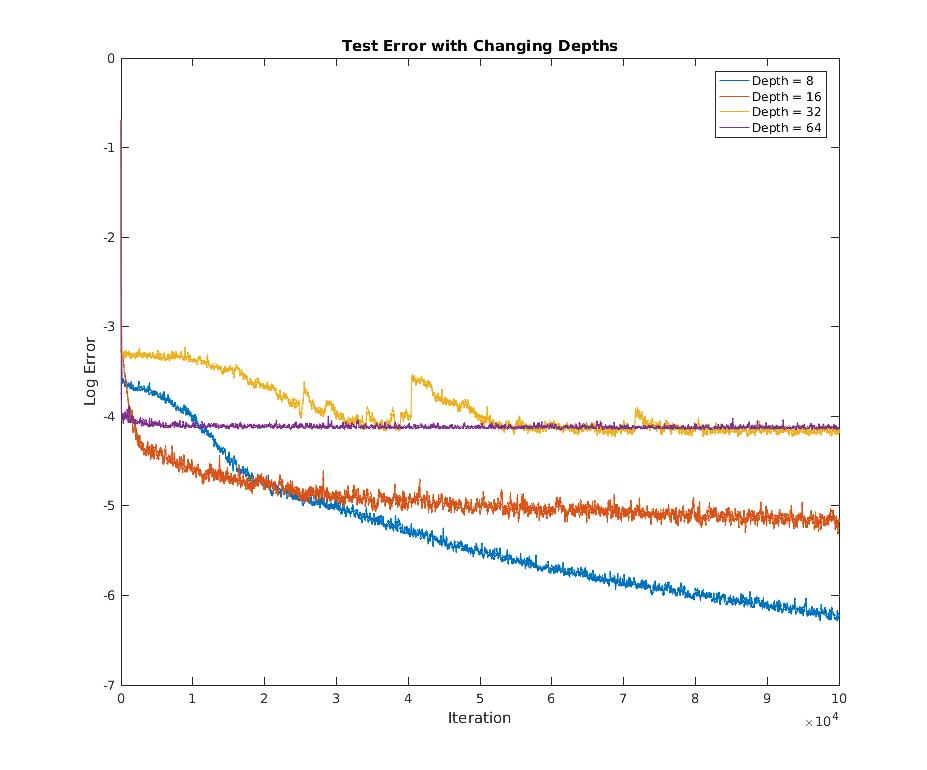
\includegraphics[height = 3in]{plotChangeDepth.jpg}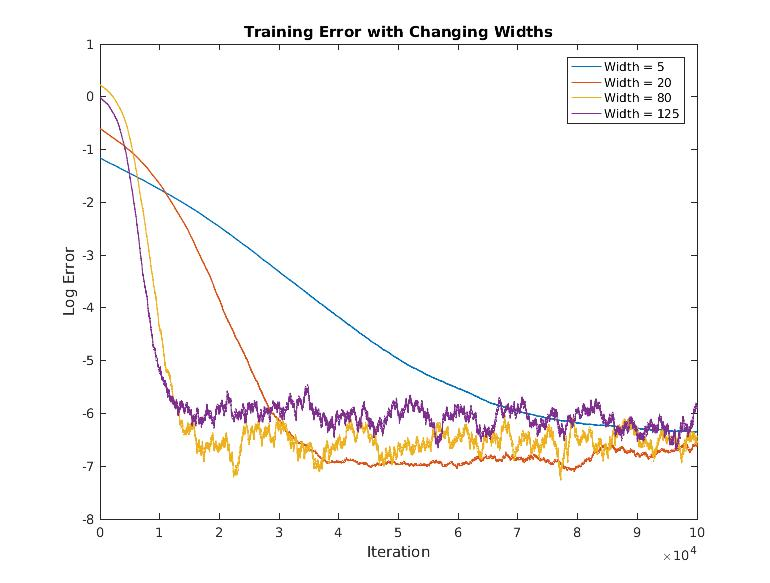
\includegraphics[height = 3in]{plotChangeWidth.jpg}
\caption{Left:Test Error of Networks of Varying Depth. Right: Test Error of Networks of Varying Width.}
\end{figure}

We note that we have been using training error as a measure of success, but it's possible that the true underlying parameters are not learned. If our loss function were strongly convex, small training error would imply a small norm in the parameter space. For the sign activation function, we can show a related result.

\begin{restatable}{theorem}{signUnique}
\label{SignUnique}
Let $\mathcal{M} = S^{d-1}$ and $\sigma$ be the sign activation function and $b_2,...,b_k = 0$. If the loss \eqref{errLoss} at $(a,\theta)$ is less than $O(1)$, then there must exist $\theta_i$ such that $w_1^T\theta_i > \Omega(1/\sqrt{k})$.
\end{restatable}



\section{Conclusion}

In this work, we view deep learning of neural networks in the context of electron-proton dynamics and analyzed the convergence of the underlying weight parameters of the neural network using arguments inspired from physics and non-convex optimization. To do so, we first established mathematical relationship between activation functions and their corresponding potentials. Next, we interpreted gradient descent as electrodynamics under a certain potential. Finally, we discovered classes of activation functions that give rise to positive convergence results, some of which relate to very commonplace activations, such as the sign and polynomial. For these classes of depth-2 neural networks, our results imply that they are provably learnable by deep learning. Our experiments seem to imply that higher depth neural networks are not learnable. 

However, we believe that convergence results for depth-2 neural networks can be extended to even more activation functions, such as the sigmoid or the ReLU. Also, we believe these convergence results can be proven with minimal assumptions. We hope that our work is a step in the theoretical understanding of the performance of neural networks seen in practice.


\bibliographystyle{apalike}
\bibliography{biblio}


%%%%%%%%%%%%%%%%%%%%%%%%%%%%%%%%%%%%Appendix

\newpage
\appendix

\section{Realizable Potentials}
\label{realizable}

\subsection{Activation-Potential Calculations}

First define the {\it dual} of a function $f: \R \to \R$ is defined to be 

\[ \widehat{f}(\rho) = E_{X,Y \sim N(\rho)}[f(X)f(Y)]\]

where $N(\rho)$ is the bivariate normal distribution with $X, Y$ unit variance and $\rho$ covariance. This is as in \cite{DanielyFS16}.

\begin{lemma}\label{rotLem}
Let $\mathcal{M} = S^{d-1}$ and $\sigma$ be our activation function, then $\widehat{\sigma}$ is the corresponding potential function.
\end{lemma}

\begin{proof}
If $u, v$ have norm 1 and if $X$ is a standard Gaussian in $\R^d$, then note that $X_1 = u^TX$ and $X_2 = v^TX$ are both standard Gaussian variables in $\R^1$ and the covariance is $E[X_1X_2] = u^Tv$. 

Therefore, the dual function of the activation gives us the potential function.

\[E_{X}[\sigma(u^TX)\sigma(v^TX)] =
E_{X,Y \sim N(u^Tv)}[\sigma(X)\sigma(Y)] = \widehat{\sigma}(u^Tv)\]

\end{proof}

By Lemma \ref{rotLem}, the calculations of the activation-potential for the sign, ReLU, Hermite, exponential functions are given in \cite{DanielyFS16}. For the Gaussian and Bessel activation functions, we can calculate directly. In both case, we notice that we may write the integral as a product of integrals in each dimension. Therefore, it suffices to check the following 1-dimensional identities.

\[\int_{-\infty}^\infty \sqrt{2}e^{x^2/4}e^{-(x-\theta)^2}\sqrt{2}e^{x^2/4}e^{-(x-w)^2} \frac{1}{\sqrt{2\pi}} e^{-x^2/2}\, dx = \sqrt{\frac{2}{\pi}}\int_{-\infty}^\infty e^{-(x-\theta)^2}e^{-(x-w)^2} \, dx = e^{-(\theta -w)^2/2}\]

\[\int_{-\infty}^\infty (\frac{2}{\pi})^{3/4}e^{x^2/4}K_0(|x-\theta|)(\frac{2}{\pi})^{3/4}e^{x^2/4}K_0(|x-w|)  \frac{1}{\sqrt{2\pi}} e^{-x^2/2}\, dx = \int_{-\infty}^\infty \frac{2}{\pi^2}K_0(|x-\theta|)K_0(|x-w|) \, dx = e^{-|\theta -w|}\]


The last equality follows by Fourier uniqueness and taking the Fourier transform of both sides, which are both equality $\sqrt{2/\pi}(\omega^2+1)^{-1}$. 



\subsection{Characterization Theorems}

\tranReal*

\begin{proof}
Let $h(x) = \mathfrak{F}^{-1}(\sqrt{\mathfrak{F}(f)})(x)$ and this is well-defined since the fourier transform was non-negative everywhere. Now, let $\sigma(x,w) = (2\pi)^{1/4}e^{x^2/4}h(x-w)$ and by assumption, it is bounded almost everywhere. Realizability follows by checking:

\begin{align*}
    E_{X \sim N}[\sigma(X,w)\sigma(X,\theta)] &= \int_{\R^n} e^{x^2/4}h(x-w)e^{x^2/4}h(x-\theta)e^{-x^2/2} \, dx \\
    &= \int_{\R^n} h(x-w)h(x-\theta) \, dx \\
    &= \int_{\R^n} h(x)h(x-(\theta-w)) \, dx \\
    &= \mathfrak{F}^{-1}(\mathfrak{F}(h\ast h)(\theta -w)) \\
    &= \mathfrak{F}^{-1}(\mathfrak{F}(h)^2(\theta - w)) \\
    &= \mathfrak{F}^{-1}(\mathfrak{F}(f)(\theta - w)) \\
    &= f(\theta - w) \\
\end{align*}



\end{proof}




\rotReal*

\begin{proof}
By \ref{rotLem} and due to the orthogonality of hermite polynomials, if $f = \sum_i a_i h_i$, where $h_i(x)$ is the i-th Hermite polynomial, then

\[\widehat{f}(\rho) = \sum_{i} a_i^2 \rho^i\]

Therefore, any function with non-negative taylor coefficients is a valid potential function, with the corresponding activation function determined by the sum of hermite polynomials, and the sum is bounded almost everywhere by assumption.
\end{proof}



\section{Generalization Error and Iteration Bounds}
\label{finite}
 
The design and analysis of gradient descent has so far assumed that we can calculate expectations perfectly. In reality, these expectations are instead replaced with empirical means. The approximate calculation of our potential and all its derivatives with samples are justified by the generalization error bounds implied by Rademacher complexities. 

Unfortunately, we cannot directly use the Gaussian distribution as it is unbounded. Therefore, we assume that our drawing distribution is the truncated Gaussian distribution in $\R^d$ such that our samples are always bounded in $l_2$ norm by $B$. We will show that applying this truncation will not affect the expectation very much.


\begin{lemma}
\label{choppedLem}
Let $f : \R^d \to \R$ be a function such that $|f(x)| \leq c\|x\|^p$. Let $X$ be a standard Gaussian in $\R^d$. Then, there exists $B = poly(d,p,\log(1/\epsilon))$ such that 

\[ |E[f(X)] - E[f(X)| \|X\|\leq B]| \leq \epsilon\]
\end{lemma}

\begin{proof}

By standard concentration bounds and analysis, 

\begin{align*}
|E[f(X)] - E[f(X)| \|X\|\leq B]| &\leq |E[f(X){\bf 1}_{\|X\|>B}] + (1- \frac{1}{P(\|X\|\leq B)}) E[f(X){\bf 1}_{\|X\|\leq B}]|\\
&\leq E[|f(X)|{\bf 1}_{\|X\|>B}] + 2cB^pe^{-B^2/8d}
\end{align*}

Taking $B = poly(d,p,\log(1/\epsilon))$ will make the second term $< \epsilon/2$, then the first term is also bounded by:

\begin{align*}
    E[|f(X)|{\bf 1}_{\|X\|>B}] &\leq (2\pi)^d \int_B^\infty cr^pe^{-r^2/2}r^{d-1}\,dr \\
    &\leq C(2\pi)^dB^{p+d}e^{-B^2/2} < \epsilon/2
\end{align*}

\end{proof}

Next, we can appeal to the following well-cited theorems and standard techniques. For a better understanding of the notation and theorems used, we refer the refer to \cite{bartlett2002rademacher}.


\begin{theorem} (\cite{bartlett2002rademacher}) Consider a function class $\mathcal{F}$ of functions $f : \mathcal{X} \to [0,1]$. And let $ x_1,...,x_n \in \mathcal{X}$ be i.i.d. samples selected according to some distribution $\mathcal{D}$. Let the Rademacher complexity of $\mathcal{F}$ to be 

\[R_n (\mathcal{F}) = E_{x_i,\sigma_i}\left[\sup_{f \in \mathcal{F}} \left|\frac{2}{n}\sum_{i=1}^nf(x_i)\sigma_i\right|\right]\]

where $\sigma_i$ are Rademacher variables. Then, for any $n$ and $\delta \in (0,1)$, with probability at least $1-\delta$, 


\[|E_{X}[f(X)]  - \frac{1}{n}\sum_{i=1}^n f(x_i)| \leq R_n(\mathcal{F}) + \sqrt{\frac{8\ln(2/\delta)}{n}} \]

for all $f \in\mathcal{F}$ simultaneously.
\end{theorem}

For all of our polynomial time bounds, whether we are calculating the potential or its derivatives, we are interested in bounding the Rademacher complexity of the class of functions of the form $\sigma_1(x^T\theta) \sigma_2(x^Tw)$, where $\sigma_1,\sigma_2$ are scalar functions.




\begin{theorem}
Let $\mathcal{X} = \{x \in \R^d, \|x\|_2\leq B\}$ and let $\sigma_1,\sigma_2 : \R \to [-C,C]$ be $L$-Lipschitz functions. Consider the following class of functions

\[\mathcal{F}_{\sigma_1,\sigma_2} = \{x\to\sigma_1(x^T\theta) \sigma_2(x^Tw) | x\in\mathcal{X}, \theta, w \in S^{d-1}\}\]

Then, \[R_n(\mathcal{F}_{\sigma_1,\sigma_2}) \leq 48CLB\sqrt{\frac{2}{n}}\]

\end{theorem}

\begin{proof}
First, let's define a simpler function class: $\mathcal{G} = \{x\to x^T\theta  | x\in\mathcal{X}, \theta \in S^{d-1}\}$. By simple Rademacher bounds on the class of linear functions \cite{kakade2009complexity}, 
 
 \[R_n(\mathcal{G}) \leq B\sqrt{\frac{2}{n}}\]
 
Since $\sigma_1,\sigma_2$ are L-lipschitz, we apply standard structural results in \cite{bartlett2002rademacher}

\[R_n(\sigma_i\circ \mathcal{G}) \leq 2LB\sqrt{\frac{2}{n}}\]

Let $s(x) = x^2$, then $s$ is $2C$-Lipschitz when $|x|\leq C$, so 

\[R_n(s\circ \sigma_i\circ\mathcal{G}) \leq 8CLB\sqrt{\frac{2}{n}}, R_n(s\circ(\sigma_1\circ \mathcal{G} +\sigma_2\circ \mathcal{G})) \leq 32 CLB\sqrt{\frac{2}{n}}\]
 
Since $2\sigma_1(x^T\theta)\sigma_2(x^Tw) = (\sigma_1(x^T\theta)+\sigma_2(x^Tw))^2 - \sigma_1(x^T\theta)^2 - \sigma_2(x^Tw)^2$, we conclude that 
\[R_n (\mathcal{F}_{\sigma_1,\sigma_2}) \leq 48CLB\sqrt{\frac{2}{n}}\]
\end{proof}

\begin{theorem}
\label{genErrBound}
Let $\mathcal{M} = S^{d-1}$ and $L$ be as in \ref{errLoss} with potential function $\Phi$ corresponding to activation $\sigma$. Assume that $|\sigma(x)|, |\sigma'(x)|,|\sigma''(x)|, |\sigma'''(x)|$ are all $O(|x|^p)$ for some $p \leq d$.  

Then, in $poly(d^p,1/\epsilon, \log(1/\zeta))$ samples, we can compute $\hat{L}$ such that with probability $1-\zeta$, we have simultaneously $\|\widehat{L}(x) -L(x)\|, \|\nabla \widehat{L}(x) = L(x)\|, \|\nabla^2\widehat{L}(x) -\nabla^2 L(x)\| \leq \epsilon$ for all $x\in \Omega$.
\end{theorem}

\begin{proof}
We first bound the generalization error of each $\Phi$. Notice that our approximation to $\Phi$ is done by first drawing $n$ i.i.d. samples $x_i \sim \mathcal{D}_B$, where $\mathcal{D}_B$ is the Gaussian in $\R^d$ truncated by the ball of radius $B = poly(d,p,\log(1/\epsilon))$. Then, we calculate the empirical average.

\[\widehat{\Phi}(\theta,w) = \frac{1}{n}\sum_{i=1}^n \sigma(x_i^T\theta)\sigma(x_i^Tw) \]

Since $|x_i^T\theta|\leq B$, we conclude that $\sigma, \sigma'$ is bounded by $poly(B^p)$. Therefore, by our error bound theorems and by simple union bounds over the $poly(k) = poly(d)$ sum of $\Phi$, we conclude that with probability $1-\zeta$, if we choose $n = poly(d^p,1/\epsilon, \log(1/\zeta))$, we have 

\[|E_{X\sim \mathcal{D}_B}[\sigma(X^Tw)\sigma(X^T\theta)] - \widehat{\Phi}(\theta^Tw)| \leq \epsilon/2\]

for all $\theta, w \in \mathcal{M}$. And combining with Lemma \ref{choppedLem}, we conclude that $|\widehat{\Phi}(\theta,w) - \Phi(\theta,w)|\leq \epsilon$. We proceed with the same proof for the first and second derivatives and use a union bound to derive our claim.
\end{proof}

\subsection{Infinite Iteration Bounds} 
\label{InfIter}


\begin{theorem}\cite{lee2016gradient}\cite{PanageasP16}\label{convStrict}
Let $f :\Omega \to \R$ be a twice differentiable function such that $\sup_{x \in \Omega} \|\nabla^2 f\| \leq L$. Let $\mathcal{S} \subseteq \Omega$ be the set of critical points of $f$ that are not local minima. Also, if $g(x) = x - \frac{1}{2L} \nabla f(x)$, then $g(\Omega) \subseteq \Omega$. 

Then, running Algorithm \ref{GD} with gradient input $\nabla f$ and stepsize $\alpha = 1/(2L)$, as the iteration  $T \to\infty$, will converge to a point $x_\infty$ outside of $S$ almost surely over randomly chosen initial points $x_0$. 
\end{theorem}

\begin{corollary}
Assume all the assumptions of Theorem \ref{convStrict} and let $f$ admit a global minima in $\overline{\Omega}$. Assume all critical points of $f$ in $\Omega$ are not local minima, except at the global minima. Then, running Algorithm \ref{GD} with gradient input $\nabla f$ and stepsize $\alpha = 1/(2L)$ will converge to the global minima almost surely as the iteration count $T \to\infty$.
\end{corollary}

\subsection{Finite Iteration Bounds} 

To derive a finite iteration bound, we will apply stochastic gradient descent to our objective function and use standard martingale techniques for analysis. We will need to slightly alter the main result in \cite{GeHJY15} because we lack strong convexity assumptions. Also, we will accordingly alter the stochastic gradient descent algorithm to terminate upon finding a critical point that is $\gamma$-strict, for small $\gamma$.


\begin{algorithm}[ht]
\SetAlgoLined
\KwIn{$\widehat{L}:\mathcal{M} \to \R$; $x_0 \in \mathcal{M}$; $T\in \N$; $\alpha \in \R$; $\epsilon\in\R$}
 
  $x = x_0$\;
 \For{i=1 to T}{
   Draw $n$ uniformly on unit sphere\;
   $x = x - \alpha(\nabla \widehat{L} (x)+n)$\;
   $x = \Pi_\mathcal{M} x$\;
   
   \If{$\|\nabla\widehat{L}(x)\|\leq 2\epsilon/3$ {\bf and} $\lambda_{min}(\nabla^2\widehat{L}(x)) \geq -2\epsilon/3$}
       {\Return $x$;}
    
  }
  {\Return FAIL;}
  
  
 \caption{$x = SGD(\widehat{L}, x_0, T,\alpha,\epsilon$)}
 \label{SGD}
\end{algorithm}


\begin{theorem}\label{strongConverge}
Let $L :\Omega \to \R$ be a twice differentiable function such that $|L(x)| \leq B, \|\nabla^2 L(x)\| \leq C,\|\nabla^2f(x) -\nabla^2f(y)\| \leq \rho\|x - y\|$ for all $x,y\in\Omega$. Also, assume that we access to stochastic function $\widehat{L}$ such that $\|\widehat{L}(x) -L(x)\|, \|\nabla \widehat{L}(x) = L(x)\|, \|\nabla^2\widehat{L}(x) -\nabla^2 L(x)\| \leq \epsilon/3$ for all $x\in \Omega$.



Then, we can choose stepsize $\eta = 1/poly(d,B,C,\rho,1/\epsilon,\log(1/\zeta))$, such that with probability at least $1-\zeta$, running Algorithm \ref{SGD} on $\widehat{f}$ with stepsize $\eta$  returns a point that is in $\mathcal{M}_\epsilon$ after at most $poly(d,B,L,\rho,1/\epsilon, \log(1/\zeta))$ iterations.
\end{theorem}

\begin{proof}
If Algorithm \ref{SGD} succeeds, then by triangle inequality and our error bounds on the stochastic function $\widehat{L}$ and its derivatives, we know that $x \in \mathcal{M}_\epsilon$. So, it suffices to argue that our algorithm succeeds with high probability.

By \cite{GeHJY15} Lemma 7 and 9, we see that if $x_i \not \in\mathcal{M}_{\epsilon/3}$ for all the iterations, then in expectation, our objective function decreases by $poly(\eta)$ and by using Azuma's inequality, this occurs with probability $1-\zeta$. Since our objective function is bounded by $poly(d,B)$, we conclude that stochastic gradient descent must have encountered a point $x_i$ such that $x_i \in \mathcal{M}_{\epsilon/3}$ after at most $poly(d,B,L,\rho,1/\epsilon,1/\gamma, \log(1/\zeta))$. Then, by our bounds on $\widehat{L}$ and $L$, we conclude that both $\|\nabla\widehat{L}(x_i)\| \leq 2\epsilon/3$ and $\lambda_{min}(\nabla^2 \widehat{L}(x_i)) \geq -2\epsilon/3$. So, our algorithm succeeds with probability $1-\zeta$.

\end{proof}



\section{Convergence of Almost Strictly Subharmonic Potentials}\label{App:Subharm}




We show convergence of a specific function $\Phi(\theta, w) = e^{-\|\theta - w\|^2/2}$, highlighting the main ideas in this specific case.

\gaussStrict*

\begin{proof}
Consider again a correlated movement, where each $\theta_i$ are moved along the same direction $v$. As before, this drops the pairwise $\theta_i$ terms, so since $O(d) > \|\theta_i -w_j\|^2 > 2d$, we see that $\Delta_{\theta_i} \Phi = (\|\theta_i -w_j\|^2 - d)\Phi(\theta_i,w_j) > e^{-O(d)}$. 

\[\Tr(\nabla^2 L) = -2\sum_{i=1}^k \sum_{j=1}^k \Delta_{\theta_i}\Phi(\theta_i, w_j) < -e^{-O(d)}\]

Therefore, $\nabla^2 L$ must admit a strictly negative eigenvalue that is less than $e^{-c_3 d}$, which implies our claim (we drop the $poly(d,k)$ terms).\\

Now, we proceed with the convergence proof. Consider the gradient descent output of the first node $\theta_1$. The loss function is given by:

\[L(\theta_1) =  - 2\sum_{j=1}^k \Phi(\theta_1,w_j)\]

By standard Chernoff bounds, we have $\|w_i\|^2 < 3cd$ for all $i$ and $\|w_i -w_j\|^2 \in (1.5cd, 2.5cd)$ for all $i, j$ with high probability as $k = poly(d)$. We just need to consider $\Omega = \{ x \in \R^d | \|x \|^2 < 3cd\}$ since the convex hull of $w_i$ is contained in $\Omega$ and so the gradient operator $g$ satisfy $g(\Omega) \subseteq \Omega$ (the gradient outside the convex hull points towards the convex hull).  

To use Thm \ref{strongConverge}, we check the regularity conditions: note that we can choose $L, B, \rho$ to be $poly(d)$ since the first, second and third partials of $\Phi$ are all bounded by $poly(d)$. Now, by choosing $\epsilon = e^{-O(d)}$ for some $c$, we know that with high probability, running SGD in $T = e^{O(d)}$ iterations will output $\theta_1$ such that 1) $\|\nabla L (\theta_1)\| < e^{-O(d)}$ and 2) $\lambda_{min}(\nabla^2L(\theta_1)) > -e^{-O(d)}$.

WLOG, $w_1$ be a closest point to $\theta_1$. Since  $\lambda_{min}(\nabla^2L(\theta_1)) > -e^{-O(d)}$, by the first part of our claim, $\|w_1 - \theta_1\|^2 < 1.1d$ and from triangle inequality, $\|w_i - \theta_1 \|^2 > c*d$ for all $i \neq 1$. 

Next, we calculate the gradient value at $\theta_1$, 

\[\|\nabla L(\theta_1)\| = \|2\sum_{j=1}^k \nabla_{\theta_1}\Phi(\theta_1,w_j)\|\]

\[ \geq \|\nabla_{\theta_1} \Phi(\theta_1,w_1) \| - \|\sum_{j>1} \nabla_{\theta_1}\Phi(\theta_1,w_j)\|\]

\[\geq \|\theta_1-w_1\|e^{-1.1d} - kc^2e^{-cd} \geq e^{-O(d)}\]

Therefore, $\epsilon = e^{-O(d)}$ can be chosen small enough to ensure that $\|\theta_1 - w_1\| = e^{-O(d)}$. \\

Finally, we proceed by induction. Since $\theta_1, w_1$ are paired to high accuracy, we note that we can treat it as if $w_1, \theta_1$ are removed from our loss equation. Therefore, we conclude that for all $\theta_i$, it will match with some $w_{\pi(i)}$ for some permutation $\pi$, with error $e^{-O(d)}$. 

\end{proof}




\section{Convergence of Almost $\lambda$-Harmonic Potentials}\label{App:EigenFunc}




First, we need some control on the size of the squares of variable charges, $a_i^2$. Node-wise gradient descent allows us to maintain that control.

\begin{theorem}\label{nonDecrease}
Let $\Phi(\theta, w)$ be $poly(d)$-Lipschitz in $\theta$, $|\Phi| \leq poly(d)$, and $\sum_{j \neq i} |a_i| + \sum_i |b_i| \leq poly(d)$. Also, assume that if $\theta_i$ is drawn uniformly on $\mathcal{M}$, 

\[E_{\theta_i}\left[\left(  \sum_{j\neq i} a_j \Phi(\theta_i,\theta_j) + \sum_{j=1}^k b_j \Phi(\theta_i,w_j)\right)^2\right] \geq \epsilon \]

Then, with probability $1-\zeta$, running Algorithm \ref{NodeGDOpt} on $\widehat{L}$ with stepsize at most $1/poly(d)$ will enforce that $a_i^2 = \Omega(\epsilon)$ when running SGD on $\theta_i$.
\end{theorem}

\begin{proof}
We want to show that $a_i^2 = \Omega(\epsilon)$. First, we analyze the random drawing of $\theta_i$. Let 

\[  C(\theta_i) = \sum_{j\neq i} a_j \Phi(\theta_i,\theta_j) + \sum_{j=1}^k b_j \Phi(\theta_i,w_j)\]

By assumption, we know that $E[C(\theta_i)^2] \geq \epsilon$. Since $a_i,b_i, \Phi$ is $poly(d)$-bounded, then $C(\theta_i)$ is $poly(d)$-bounded and is therefore a $poly(d)$ sub-Gaussian variable. From standard concentration bounds, we see that after $poly(d,1/\epsilon)$ samples, we can find $\theta_i$ such that $C(\theta_i)^2 \geq \epsilon/2$. 


Next, notice that $\hat{L}$ is a quadratic in $a_i$, so the gradient step on $a_i$ will optimize $a_i = a_i^*(\theta_i)$. 

By optimality of $a^*$, 

\begin{equation}
0 = \pd{\hat{L}}{a_i} = 2a_i \widehat{\Phi}(\theta_i,\theta_i) + 2\sum_{j\neq i} a_j \widehat{\Phi}(\theta_i,\theta_j) + 2\sum_{j=1}^k b_j \widehat{\Phi}(\theta_i,w_j)
\end{equation} 

Therefore, 

\[ a_i^* = - \frac{1}{\widehat{\Phi}(\theta_i,\theta_i)} (\sum_{j\neq i} a_j \widehat{\Phi}(\theta_i,\theta_j) + \sum_{j=1}^k b_j \widehat{\Phi}(\theta_i,w_j)) = -\frac{1}{\widehat{\Phi}(\theta_i,\theta_i)}\widehat{C}(\theta_i) \]


By our generalization bounds, in $poly(d,1/\epsilon)$ samples, we can find $\theta_i$ such that $\widehat{C}(\theta_i)^2 \geq \epsilon/4$ (notice $\Phi(\theta_i,\theta_i) = 1$). Since $a_i = 0$, we conclude that we can find $\theta_i$ such that 

\[(\pd{\hat{L}}{a_i})^2 = 4 \widehat{C}(\theta_i)^2 \geq \epsilon\]

Therefore, after $poly(d,1/\epsilon)$, our sampling algorithm will return $\theta_i$ such that $a_i^2 = a_i^*(\theta_i)^2 \geq \epsilon /4$. \\

Next, we examine the SGD steps. Note

\begin{equation}
\nabla_{\theta_i} \widehat{C}(\theta_i) =  \sum_{j\neq i} a_j \nabla_{\theta_i}\widehat{\Phi}(\theta_i,\theta_j) + \sum_{j=1}^k b_j \nabla_{\theta_i}\widehat{\Phi}(\theta_i,w_j) = \frac{1}{2a_i^*} \nabla_{\theta_i}\widehat{L}
\end{equation}

Now, we calculate the following gradient: 

\begin{equation}
\nabla_{\theta_i} (a_i^*)^2 = 2a_i^*\frac{-1}{\widehat{\Phi}(\theta_i,\theta_i)} \nabla_{\theta_i} \widehat{C}(\theta_i) = \frac{1}{\widehat{\Phi}(\theta_i,\theta_i)} (-\nabla_{\theta_i} \widehat{L})
\end{equation}

Therefore, since $\theta_i$ moves in the direction of the gradient of $(a_i^*)^2$ in expectation and $(a_i^*)^2$ is $poly(d)$-Lipschitz in $\theta_i$, so we conclude by standard gradient descent analysis that $(a_i^*)^2$ is a supermartingale. Finally, we can conclude with Azuma's, that in $poly(1/\epsilon,d,\log(1/\zeta))$ iterations, $(a_i^*)^2 = \Omega(\epsilon)$ with probability $1-\zeta$ .\\


\end{proof}


\eigConv*

\begin{proof}
We start with the construction. Let $u,v$ be on the unit sphere, and WLOG let $v = (0,...,1)$. Then, we can reparametrize any function of the dot product $f(u^Tv) = f(cos(\theta))$, where $\theta \in [0, \pi]$ is the angle between $u$ and the positive $z$-axis.
Using the Laplacian formula on $S^{d-1}$ gives:

\[\Delta f = (\sin \theta)^{2-d} \frac{\partial}{\partial \theta}\left[ (\sin \theta)^{d-2} \frac{\partial f(\cos \theta)}{\partial \theta}\right] = f''(\cos\theta)(\sin \theta)^{2} - (d-1)\cos(\theta)f'(\cos\theta)\]

We want $f$ to be approximately $1$-harmonic, so we want to approximately solve:

\[f''(x)(1-x^2) - (d-1)xf'(x) =  f(x) \]

Let us construct our approximate function $f$ as follows. Let $c_n$ are the Taylor coefficients of $f(x)$, then we want to solve the equation:
Therefore, we get the following recurrence: $c_n (n(n-1) + (d-1)*n + 1) = c_{n+2} (n+2)(n+1)$. Let $c_0 = 1, c_1 = 0$, then we run this recurrence holds $n=0,...,N-2$ for some $N$ even and set $c_{N+i} = 0$ for $i > 0$, then

\[\Delta f = f''(\cos\theta)(\sin \theta)^{2} - (d-1)\cos(\theta)f'(\cos\theta) = f(\cos(x)) + k_Nx^N\]

Where $k_N = N^2 + (d-2)N + 1$. Notice that $f(x)$ has non-negative Taylor coefficients and is a bounded polynomial, so $f$ is a realizable potential function. \\

We show our result under this potential function $\Phi = f$. Our objective function is:

\[L(a, \theta) = 2\sum_{i=1}^n \sum_{j=1}^n a_i b_j \Phi(\theta_i^T w_j) + \sum_{i=1}^n \sum_{j\neq i} a_i a_j\Phi(\theta_i^T\theta_j)  +\sum_{i=1}^n a_i^2\Phi(1)  \]

Assume that $(a, \theta) \in \mathcal{M}_{\epsilon^2/(4d)}$ and we have a $(a_i,\theta_i)$ that does not satisfy (i), (ii), (iii). Then,

\[|\pd{L}{a_i}| = |2\sum_{j=1}^n  b_j  \Phi(\theta_i^T w_j) +  2\sum_{j\neq i} a_j \Phi(\theta_i^T\theta_j)  + 2a_i\Phi(1)| \leq \epsilon \] 

And, 

\[\Delta_{\theta_i} L =  2\sum_{j=1}^n a_i b_j  (-\Phi(\theta_i^T w_j) + k_N(\theta_i^Tw_j)^N) +  2\sum_{j\neq i} a_i a_j(-\Phi(\theta_i^T\theta_j) + k_N(\theta_i^T\theta_j)^N)\]

Therefore,

\[|\Delta_{\theta_i}L + 2a_i^2\Phi(1)| \leq \epsilon |a_i| +  2|a_i| k_N|\sum_{j=1}^n b_j (\theta_i^Tw_j)^N +  \sum_{j\neq i}  a_j(\theta_i^T\theta_j)^N|\]

Since (i), (ii) does not hold and $\|a\|\leq \poly(d)$, we can choose $N = O(\frac{1}{\epsilon}\log(d))$ large enough such that 

\[ 2k_N |\sum_{j=1}^n b_j (\theta_i^Tw_j)^N +  \sum_{j\neq i}  a_j(\theta_i^T\theta_j)^N| \leq  2poly(d,k,N)e^{-\epsilon N} \leq \epsilon/2\] 

Therefore, by (iii) and $\Phi(1) > 1$,

\[\Delta_{\theta_i} L \leq -2a_i^2 \Phi(1) +\epsilon |a_i|+(\epsilon/2)|a_i| \leq |a_i|(-2\epsilon \Phi(1) + 3\epsilon/2) \leq -\epsilon^2/4\]

This implies that $(a,\theta)$ is $\epsilon^2/(4d)$-strict, contradicting that it is in $\mathcal{M}_{\epsilon^2/(4d)}$. \\

Finally, we proceed with the convergence proof. Consider the initialization of $\theta_1$. If the sampling fails, then by Theorem \ref{nonDecrease}, with high probability we have

\[ E\left[\left( \sum_{j < 1} a_j \Phi(\theta_i,\theta_j) + \sum_{j=1}^k b_j \Phi(\theta_i,w_j)\right)^2\right] < \epsilon\]

Otherwise, the theorem allows us to deduce that throughout the SGD algorithm applied on $\theta_1$, $a_1 = \Omega(\epsilon)$. To use Theorem \ref{strongConverge}, we check the regularity conditions. Since $\mathcal{M} = S^{d-1}$, then we can choose $B, L, \rho$ to be $poly(d)$ since $\Phi$ and the second and third partials of $\Phi$ are all bounded by $poly(d)$. Furthermore, by our construction, our activation function $\sigma$ and its derivatives are bounded in magnitude by $|x|^{O(\log(d)/\epsilon)}$. By Theorem \ref{genErrBound}, with high probability, we can construct a stochastic oracle up to $\epsilon$ error with sample complexity $poly(d^{\log (d)/\epsilon},1/\epsilon)$.


Therefore, we conclude that we converge to $\theta_1 \in \mathcal{M}_{\epsilon^2/(4d)}$. By the first part of this theorem, since $|a_i| = \Omega(poly(\epsilon))$, this implies that it is in an $\epsilon$-neighborhood of some $w_{i}$ in $poly(d,1/\epsilon)$ time. Furthermore, note that $|a_1| \leq poly(d)$ by using the explicit formula.

Now, we proceed with induction and repeat the same argument on $\theta_2$ and so on. The only subtlety is that $\theta_2$ could be in an $\epsilon$-neighborhood of $\theta_1$. However, by the optimality of $a_1$, we note that $a_2^*(\theta_2) = 0$ if $\theta_2 =\theta_1$. Since $a_2^*$ is $poly(d)$-Lipschitz and $a_2^2 = a_2^*(\theta_2)^2$ is bounded below by $\Omega(\epsilon)$, we conclude that $\theta_2$ cannot be close to $\theta_1$ but converges to a point close to $w_{j}$, $j\neq i$. By applying this logic to all $\theta_i$, we deduce that $\theta$ is within $\epsilon$ of the global minima.

\end{proof}


\section{Convergence of Polynomial Potentials}


\polyConv*

\begin{proof}
Without loss of generality let $w_1,...,w_k$ be the standard basis vectors $e_1,..,e_k$. and these basis vectors span the whole optimization space. Consider the algorithm on just the first node: $(a_1,\theta_1)$. For simplicity, we will drop the subscripts in the proof. 

First, consider the initialization of $\theta$, notice that upon initialization and optimization, if $\theta$ is drawn from a standard Gaussian, then by independence and $E[\theta_i] = 0$,

\[E[C(\theta)^2] = E\left[\left(\sum_{i=1}^k  b_i (\theta_i)^l\right)^2\right] = \sum_{i=1}^k b_i^2E[\theta_i^{2l}]\]

There must exists $j$ such that $|b_j|\geq 1$ and since drawing $\theta_i$ uniformly on $S^{d-1}$ is just a $poly(d)$ rescaling of a Gaussian, we conclude that $E[a^2]\geq1/poly(d)$. By Theorem \ref{nonDecrease}, we conclude that $E[a^2] \geq 1/poly(d)$ throughout the gradient descent algorithm. Next, to use Theorem \ref{strongConverge}, we check the regularity conditions. By assumption, we can choose $B, L, \rho$ to be $poly(d)$ since $\Phi$ and the second and third partials of $\Phi$ are all bounded by $poly(d)$ in $\Omega$. Furthermore, our activation function $\sigma$ and its derivatives are bounded in magnitude by $|x|^{l}$, where $l$ is fixed. By Theorem \ref{genErrBound}, with high probability, we can construct a stochastic oracle up to $\epsilon$ error with sample complexity $poly(d,1/\epsilon)$.


Therefore, we conclude that we converge to $\theta \in \mathcal{M}_{poly(\epsilon,1/d)}$ in $poly(d,1/\epsilon)$ iterations. Note that this is a constrained optimization problem, so by introducing a Lagrange multiplier $\lambda$, the optimality conditions are:

\[|\pd{L}{a}| = |2\sum_{i=1}^k b_i (\theta_i)^l + 2a| \leq poly(\epsilon,1/d)\]

\[ |(\nabla_\theta L)_i| = |\theta_i||2ab_il(\theta_i)^{l-2}  -2\lambda| \leq poly(\epsilon,1/d)  \]

where $\lambda$ is chosen that minimizes 

\[\lambda = \arg \min_\lambda \sum_i (ab_i l (\theta_i)^{l-1} - \lambda\theta_i)^2 = \sum_i ab_i l (\theta_i)^l = -la^2 + poly(\epsilon,1/d) \]


Therefore, either $|\theta_i| \leq poly(\epsilon,1/d)$ or $|2ab_il(\theta_i)^{l-2} - 2 \lambda |\leq poly(\epsilon,1/d)$. Next, the projected Hessian is a diagonal matrix with diagonal entry: 

\[(\nabla^2 L)_{ii} = 2a b_i l(l-1)(\theta_i)^{l-2} - 2 \lambda\]

Assume that there exists $\theta_i, \theta_j$ such that $|\theta_i|,|\theta_j| \geq poly(\epsilon,1/d)$, then we conclude that the other inequality must hold for coordinates $i, j$. So,

\[(\nabla^2 L)_{ii} = 2a b_i l(l-1)(\theta_i)^{l-2} - 2 \lambda \leq 2(l-2)\lambda + (l-1)\epsilon \leq -2(l-2)la^2 + poly(\epsilon,1/d)\]

Since $l-2 \geq 1$ and $a^2 \geq 1/poly(d)$, we conclude that there exists a vector with $v_k = 0$ for all $k\neq i, j$ such that $v^T\theta = 0$ (in the tangent space) and $v^T(\nabla^2 L) v  = -2(l-2)l a^2 + poly(\epsilon,1/d) < -poly(\epsilon,1/d)$. This contradicts $\theta \in \mathcal{M}_{poly(\epsilon,1/d)}$, so $\theta$ is in some $\epsilon$ neighborhood of some $w_j$. Furthermore, note that $|a_1| \leq poly(d)$ and there exists $b_j$ such that $|b_j| \geq 1$ as some $w_i$ has not yet been paired with a $\theta$.

So we can proceed with induction and repeat the same argument on the second node $\theta_2$ and so on. Since $\theta_1$ is matched to some $w_i$, note that we can treat $\theta_1$ as $w_i$ up to some $poly(\epsilon,1/d)$ error term. Furthermore, $\theta_2$ will not converge to $w_i$ because by the optimality of $a_1$, we note that $a_2^*(\theta_2) = 0$ if $\theta_2 =\theta_1$. Since $a_2^*$ is $poly(d)$-Lipschitz and $a_2^2 = a_2^*(\theta_2)^2$ is bounded below by $\Omega(\epsilon)$, we conclude that $\theta_2$ cannot be close to $\theta_1$ but converges to a point close to $w_{j}$, $j\neq i$. By applying this logic to all $\theta_i$, we deduce that $\theta$ is within $\epsilon$ of the global minima.

\end{proof}


\section{Proof of Sign Uniqueness}


\signUnique*

\begin{proof}
WLOG let $w_1 = e_1$. Notice that our loss can be bounded below by Jensen's:

\[E_X \left[ \left( \sum_{i=1}^k a_i \sigma(\theta_i^TX) - \sigma(X_1)\right)^2 \right] \geq E_{X_1} \left[ \left( E_{X_2...X_d}\left[ \sum_{i=1}^k a_i \sigma(\theta_i^TX) \right]- \sigma(X_1)\right)^2 \right]
\]

where $X$ is a standard Gaussian in $\R^d$. 

\begin{align*}
E_{X_2,..,X_d} \left[  \sum_{i=1}^k a_i \sigma(\theta_i^TX) \right] &= \sum_{i=1}^k a_i E_{X_2,...X_d}\left[  \sigma(\theta_{i1}X_1 + \sum_{j >1} \theta_{ij}X_{j})  \right]\\
&= \sum_{i=1}^k E_{Y} \left[   \sigma(\theta_{i1}X_1 + \sqrt{1-\theta_{i1}^2}Y)  \right]  \\
&= \sum_{i=1}^k a_i E_{Y} \left[   \sigma(\textstyle\frac{\theta_{i1}}{\sqrt{1-\theta_{i1}^2}}X_1 + Y)  \right] 
\end{align*}

where $Y$ is an independent standard Gaussian and for any small $\delta$, if $p(y)$ is the standard Gaussian density, 

\[ E_Y[\sigma(\delta + Y)] = \int_{-\delta}^{\delta} p(y) \, dy = 2p(0)\delta + O(\delta^2) \]

If $w_1^T\theta_i = \theta_{i1} < \epsilon$ for all $i$, then notice that with high probability on $X_1$ (say condition on $|X_1| \leq 1$), 

\[E_{Y} \left[   \sigma(\textstyle\frac{\theta_{i1}}{\sqrt{1-\theta_{i1}^2}}X_1 + Y)  \right] = 2p(0)\textstyle\frac{\theta_{i1}}{\sqrt{1-\theta_{i1}^2}}X_1 + O(\epsilon^2X_1^2)\]

Therefore, since $\epsilon < O(1/\sqrt{k})$,

\[E_{X_2,..,X_d} \left[  \sum_{i=1}^k a_i \sigma(\theta_i^TX) \right]  = X_1 \sum_{i=1}^k2p(0)a_i\textstyle\frac{\theta_{i1}}{\sqrt{1-\theta_{i1}^2}} + O(k\epsilon^2X_1^2) = cX_1+O(1)\] 


Finally, our error bound is now

\[E_{X_1} \left[ \left( E_{X_2...X_d}\left[ \sum_{i=1}^k a_i \sigma(\theta_i^TX) \right]- \sigma(X_1)\right)^2 \right] \geq E_{|X_1| \leq 1}[(cX_1+O(1) - \sigma(X_1))^2]\]

And the final expression is always larger than some constant, regardless of $c$.
\end{proof}






\end{document}

 